\documentclass[aspectratio=169]{beamer}

\usepackage[T5]{fontenc}
\usepackage[utf8]{inputenc}
\usepackage{lmodern}

\usetheme{Madrid}

\usepackage{graphicx}
\usepackage{multicol}
\usepackage{amsmath,amssymb}

% Outline look: blue text, numbered, no balls
\setbeamertemplate{section in toc}{%
  \leavevmode\inserttocsectionnumber.~\inserttocsection\par}
\setbeamercolor{section in toc}{fg=blue}

\hypersetup{colorlinks=true, urlcolor=blue}

\newcommand{\backbtn}{%
  \hfill\hyperlink{outline}{\beamerbutton{Mục lục}}}


% Giảm khoảng cách trên/dưới công thức hiển thị để slide gọn hơn
\makeatletter
\def\tight@disp{\setlength\abovedisplayskip{4pt plus 2pt}%
  \setlength\belowdisplayskip{4pt plus 2pt}%
  \setlength\abovedisplayshortskip{2pt plus 1pt}%
  \setlength\belowdisplayshortskip{2pt plus 1pt}}
\g@addto@macro\normalsize{\tight@disp}
\g@addto@macro\small{\tight@disp}
\g@addto@macro\footnotesize{\tight@disp}
\g@addto@macro\scriptsize{\tight@disp}
\makeatother

\title[Giới thiệu]{Giới thiệu: Khái niệm về ứng suất}
\author[© N. V. Sỹ]{Nguyễn Văn Sỹ}
\institute[TNUT]{%
  Bộ môn Hệ thống Công nghiệp \\
  Trường Đại học Kỹ thuật Công nghiệp \\
  \href{mailto:vansy@tnut.edu.vn}{vansy@tnut.edu.vn}}
\date[Cơ học vật liệu]{\large Cơ học vật liệu – Khái niệm về ứng suất \\[0.5em] \footnotesize \copyright\ Nguyễn Văn Sỹ}

\begin{document}

\begin{frame}
  \titlepage
\end{frame}
%====================
\begin{frame}{Tài liệu tham khảo}
	\small
	F. P. Beer, E. R. Johnston, Jr., J. T. DeWolf, D. F. Mazurek,
	\emph{Mechanics of Materials}, 6th ed., McGraw-Hill, New York, 2012.
	
	\vspace{1em}
	\footnotesize\color{gray}
	Toàn bộ hình vẽ trong bài giảng được trích từ giáo trình trên, chỉ sử dụng
	cho mục đích giảng dạy nội bộ.
\end{frame}
% ===== OUTLINE SLIDE =====
\begin{frame}[t]{Nội dung}
  \hypertarget{outline}{}
  \tiny
  \begin{multicols}{2}
    \tableofcontents[hideallsubsections]
  \end{multicols}
\end{frame}

% ===== CONTENT SLIDES (one per entry) =====
\section{Khái niệm ứng suất}
\begin{frame}{Khái niệm ứng suất}
  \begin{itemize}
    \setlength{\itemsep}{1.2em}
    \item Mục tiêu chính của môn Cơ học vật liệu là trang bị cho
          người kỹ sư tương lai các phương pháp phân tích và thiết kế
          nhiều loại máy móc và kết cấu chịu tải.
    \item Việc phân tích và thiết kế một kết cấu đều liên quan đến
          việc xác định \emph{ứng suất} và \emph{biến dạng}.
          Chương này tập trung vào khái niệm về ứng suất.
  \end{itemize}
\end{frame}
% ===================
\section{Nhắc lại về tĩnh học}
\begin{frame}[t]{Nhắc lại về tĩnh học}
\hypertarget{s2}{}
  \begin{columns}[c]
    \column{0.5\textwidth}
      \centering
      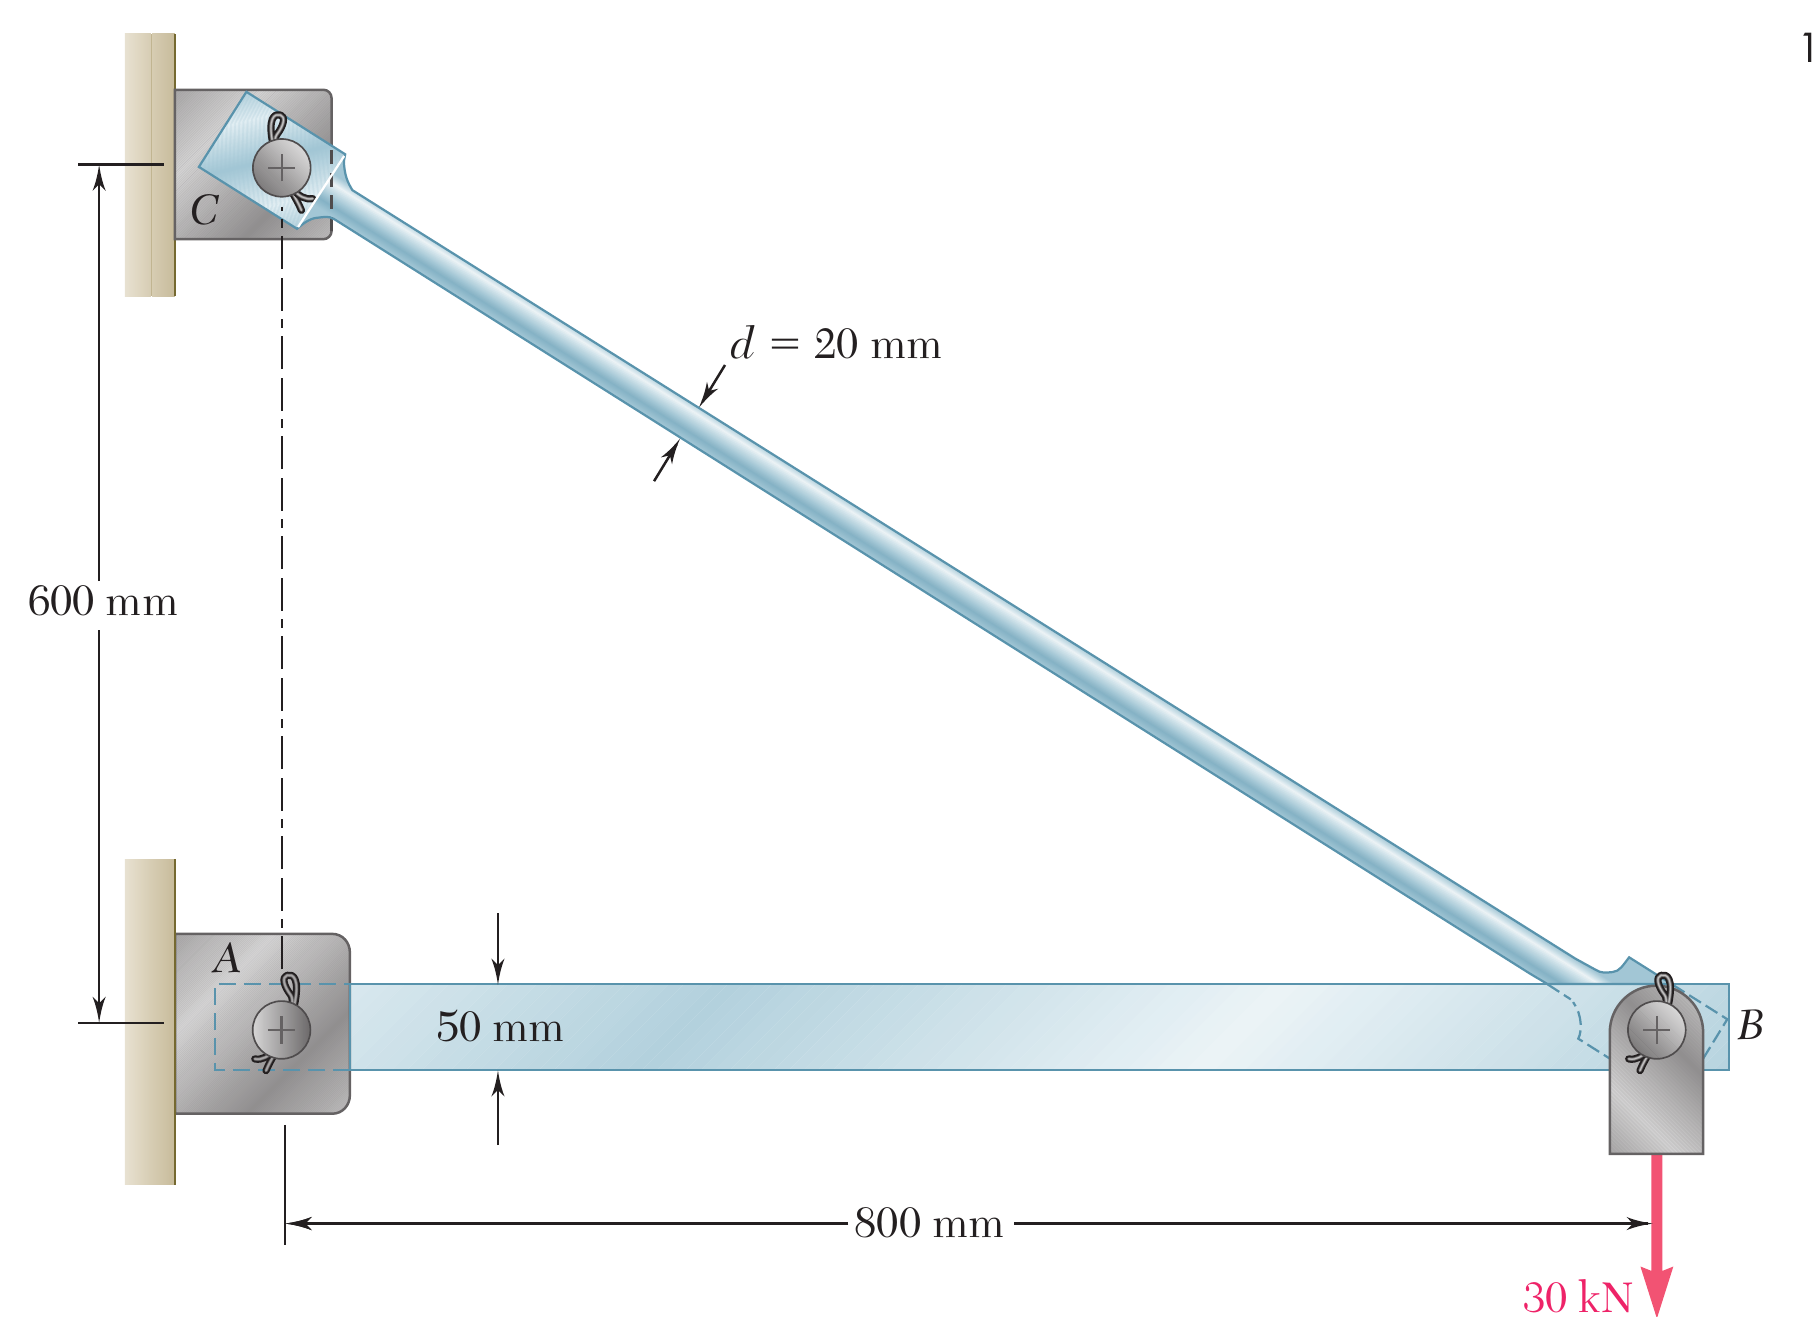
\includegraphics[width=\linewidth,height=5cm,keepaspectratio]{Chap_1/fig_1_1.png}
    \column{0.5\textwidth}
\normalsize
      \begin{itemize}
        \setlength{\itemsep}{0.8em}
        \item Kết cấu được thiết kế để chịu một tải trọng 30 kN.
        \item Kết cấu gồm một thanh dầm (boom) và một thanh giằng (rod)
              được nối với nhau bằng các chốt (liên kết không truyền mô men)
              tại các điểm nối và các gối đỡ.
        \item Thực hiện phân tích tĩnh học để xác định nội lực trong
              từng cấu kiện và các phản lực tại các gối đỡ.
      \end{itemize}
  \end{columns}
\end{frame}
% ===================
\section{Sơ đồ vật thể tự do của kết cấu}
\begin{frame}[t]{Sơ đồ vật thể tự do của kết cấu}
\hypertarget{s3}{}
  \begin{columns}[T]
    \column{0.5\textwidth}
      \centering
      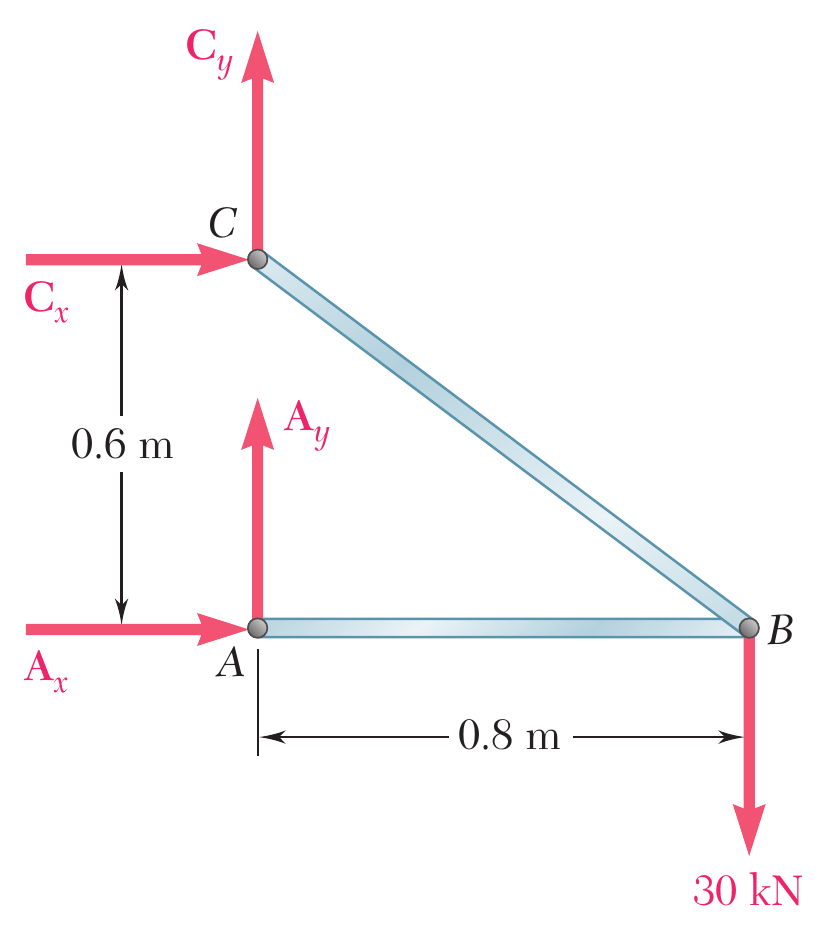
\includegraphics[width=\linewidth,height=6cm,keepaspectratio]{Chap_1/fig_1_2.png}
    \column{0.5\textwidth}
      \small
      \begin{itemize}
        \setlength{\itemsep}{0.6em}
        \item Tách kết cấu khỏi các gối đỡ, biểu diễn các tải trọng
              và phản lực.
        \item Điều kiện cân bằng tĩnh học:
        \vspace{0.3em}
        \[
          \begin{aligned}
            \textstyle \sum M_C &= 0 = A_x(0{,}6\,\mathrm{m}) - (30\,\mathrm{kN})(0{,}8\,\mathrm{m}) \\
            A_x &= 40\,\mathrm{kN} \\[0.6em]
            \textstyle \sum F_x &= 0 = A_x + C_x \\
            C_x &= -A_x = -40\,\mathrm{kN} \\[0.6em]
            \textstyle \sum F_y &= 0 = A_y + C_y - 30\,\mathrm{kN} = 0 \\
            A_y + C_y &= 30\,\mathrm{kN}
          \end{aligned}
        \]
        \item $A_y$ và $C_y$ không thể xác định được chỉ từ các
              phương trình này.
      \end{itemize}
  \end{columns}
\end{frame}
% =========================
\section{Sơ đồ vật thể tự do của từng bộ phận}
\begin{frame}[t]{Sơ đồ vật thể tự do của từng bộ phận}
\hypertarget{s4}{}
  \begin{columns}[T]
    \column{0.4\textwidth}
      \centering
      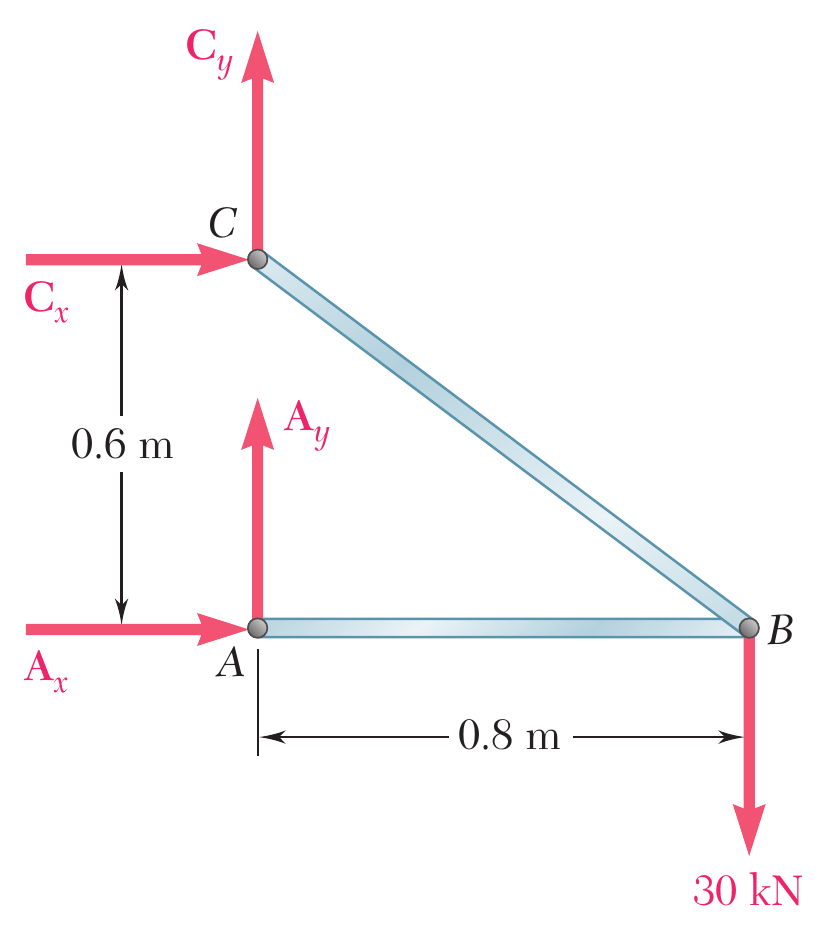
\includegraphics[width=\linewidth,height=3.5cm,keepaspectratio]{Chap_1/fig_1_2.png}\\[2pt]
      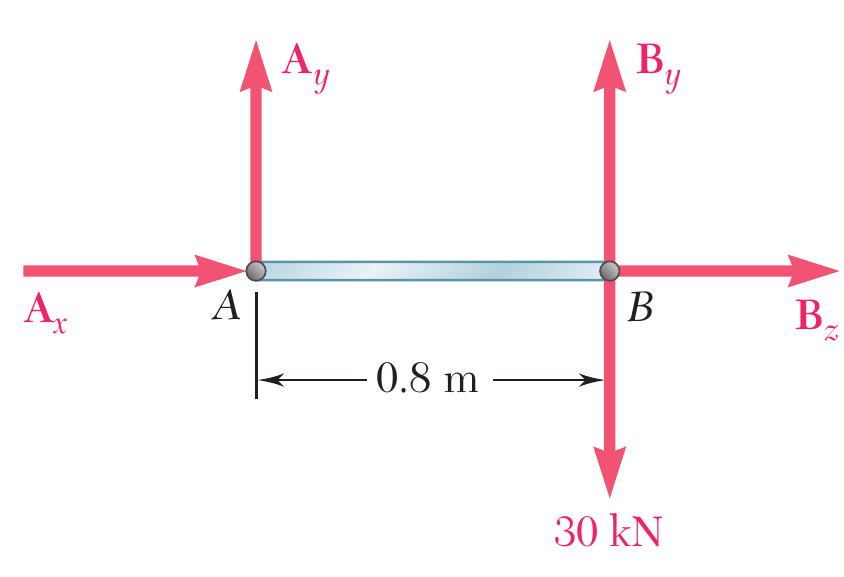
\includegraphics[width=\linewidth,height=3cm,keepaspectratio]{Chap_1/fig_1_3.png}
    \column{0.6\textwidth}
      \small
      \begin{itemize}
        \setlength{\itemsep}{0.5em}
        \item Ngoài toàn bộ kết cấu, từng bộ phận cũng phải thỏa mãn
              các điều kiện cân bằng tĩnh học.
        \item Xét sơ đồ vật thể tự do của dầm AB:
        \[          \sum M_B = 0 = -A_y(0{,}8\,\mathrm{m}); \quad A_y = 0        \]
        Thế vào phương trình cân bằng của kết cấu:
        \[          C_y = 30\,\mathrm{kN}        \]
        \item Kết quả:
        \[
        A_x = 40\,\mathrm{kN}\ \rightarrow \quad
          C_x = 40\,\mathrm{kN}\ \leftarrow \quad
          C_y = 30\,\mathrm{kN}\ \uparrow
          \]
        Các phản lực có phương dọc theo dầm và thanh giằng.
      \end{itemize}
  \end{columns}
\end{frame}
% =========
\section{Phương pháp tách nút}
\begin{frame}[t]{Phương pháp tách nút}
\hypertarget{s5}{}
  \begin{columns}[T]
    \column{0.42\textwidth}
      \centering
      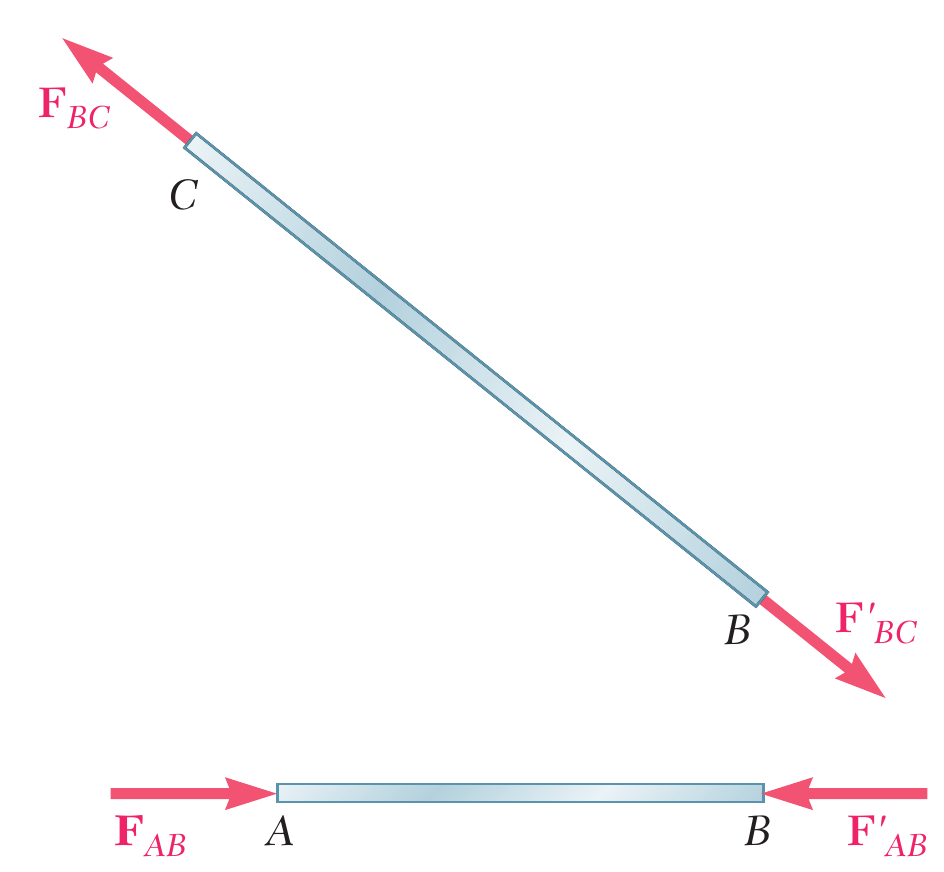
\includegraphics[width=\linewidth,height=3.5cm,keepaspectratio]{Chap_1/fig_1_5.png}\\[2pt]
      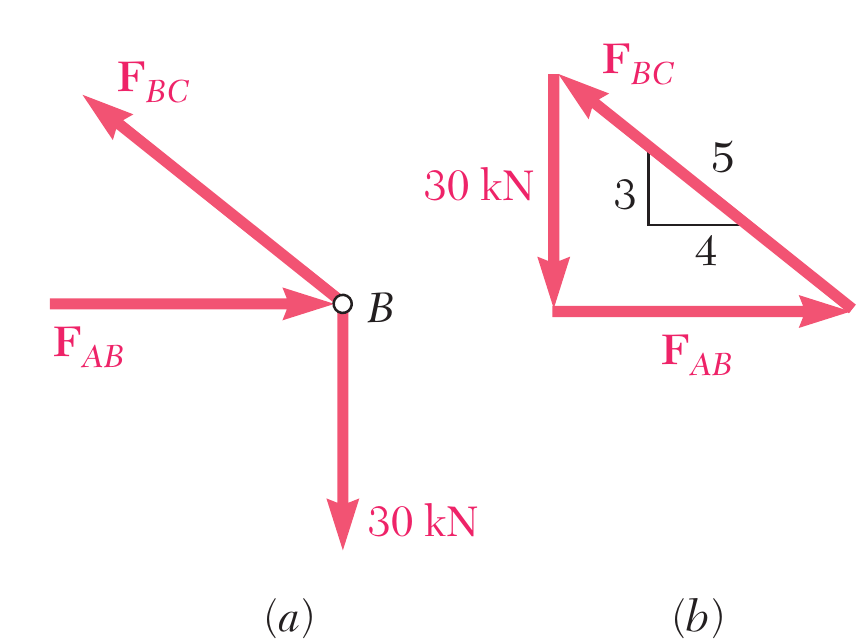
\includegraphics[width=\linewidth,height=3.5cm,keepaspectratio]{Chap_1/fig_1_4.png}
    \column{0.56\textwidth}
      \small
      \begin{itemize}
        \setlength{\itemsep}{0.8em}
        \item Dầm và thanh giằng là các cấu kiện chịu hai lực, tức là
              chỉ chịu tác dụng của hai lực đặt tại hai đầu cấu kiện.
        \item Để cân bằng, các lực phải cùng phương với đường nối hai
              điểm đặt lực, bằng nhau về độ lớn và ngược chiều nhau.
      \end{itemize}

      \vspace{0.5em}
      Các nút phải thỏa mãn điều kiện cân bằng tĩnh học, có thể biểu
      diễn dưới dạng tam giác lực:
      \[
        \textstyle\sum \vec{F}_B = 0
      \]
      \[
        \frac{F_{AB}}{4} = \frac{F_{BC}}{5} = \frac{30\,\mathrm{kN}}{3}
      \]
      \[
        F_{AB} = 40\,\mathrm{kN}, \qquad F_{BC} = 50\,\mathrm{kN}
      \]
  \end{columns}
\end{frame}
% =========
\section{Phân tích ứng suất}
\begin{frame}[t]{Phân tích ứng suất}
\hypertarget{s6}{}
  \begin{columns}[T]
    \column{0.42\textwidth}
      \centering
      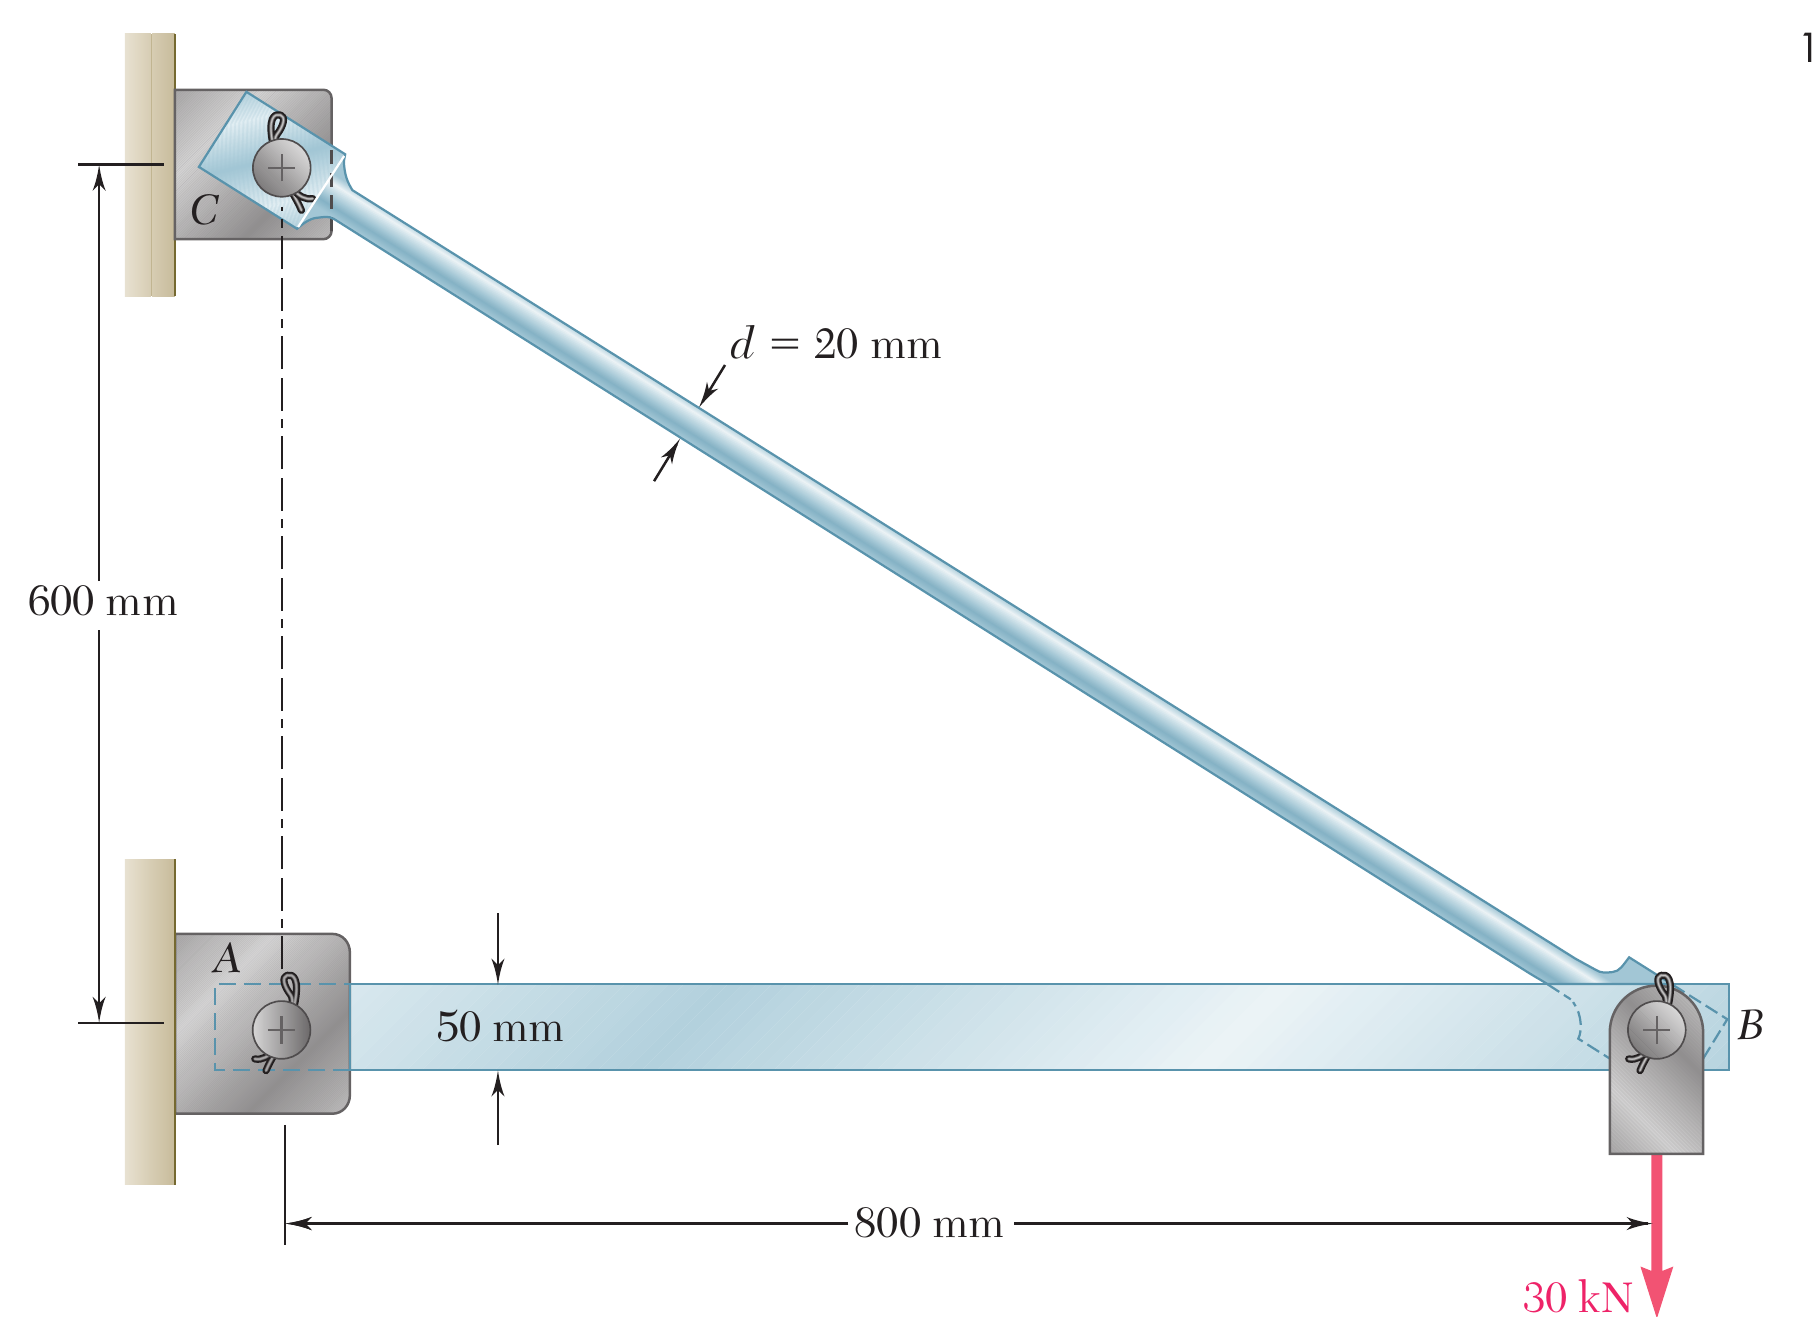
\includegraphics[width=\linewidth,height=3.5cm,keepaspectratio]{Chap_1/fig_1_1.png}
      \\[0.3em]
      $d_{BC} = 20\,\mathrm{mm}$\\[0.3em]
      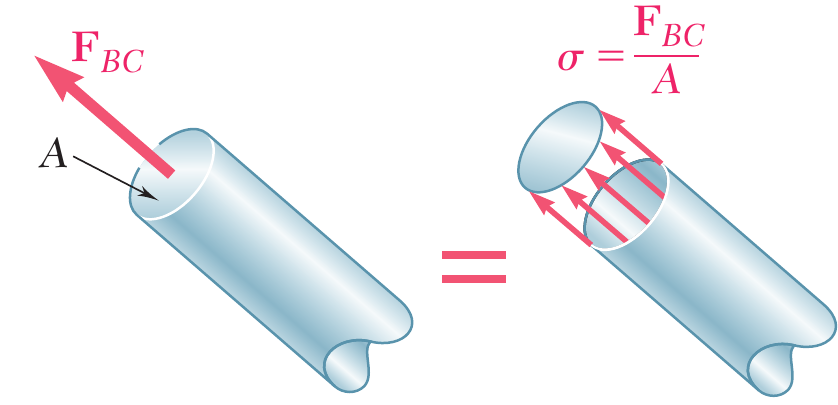
\includegraphics[width=\linewidth,height=2.6cm,keepaspectratio]{Chap_1/fig_1_7.png}
    \column{0.56\textwidth}
      \small
      Kết cấu có chịu được an toàn tải trọng 30 kN hay không?

      \begin{itemize}
        \setlength{\itemsep}{0.5em}
        \item Từ phân tích tĩnh học:
        \[
          F_{AB} = 40\,\mathrm{kN}\ \text{(nén)}, \qquad
          F_{BC} = 50\,\mathrm{kN}\ \text{(kéo)}
        \]
        \item Tại mọi mặt cắt qua thanh $BC$, nội lực là 50 kN với
              cường độ lực, hay \underline{ứng suất}, bằng:
        \[
          \sigma_{BC} = \frac{P}{A}
          = \frac{50 \times 10^{3}\,\mathrm{N}}{314 \times 10^{-6}\,\mathrm{m}^2}
          = 159\,\mathrm{MPa}
        \]
        \item Từ đặc tính vật liệu của thép, ứng suất cho phép là:
        \[
          \sigma_{\mathrm{all}} = 165\,\mathrm{MPa}
        \]
        \item Kết luận: thanh $BC$ đủ bền.
      \end{itemize}
  \end{columns}
\end{frame}
% =========
\section{Bài toán thiết kế}
\begin{frame}[t]{Bài toán thiết kế}
  \begin{columns}[T]
    \column{0.35\textwidth}
      \centering
      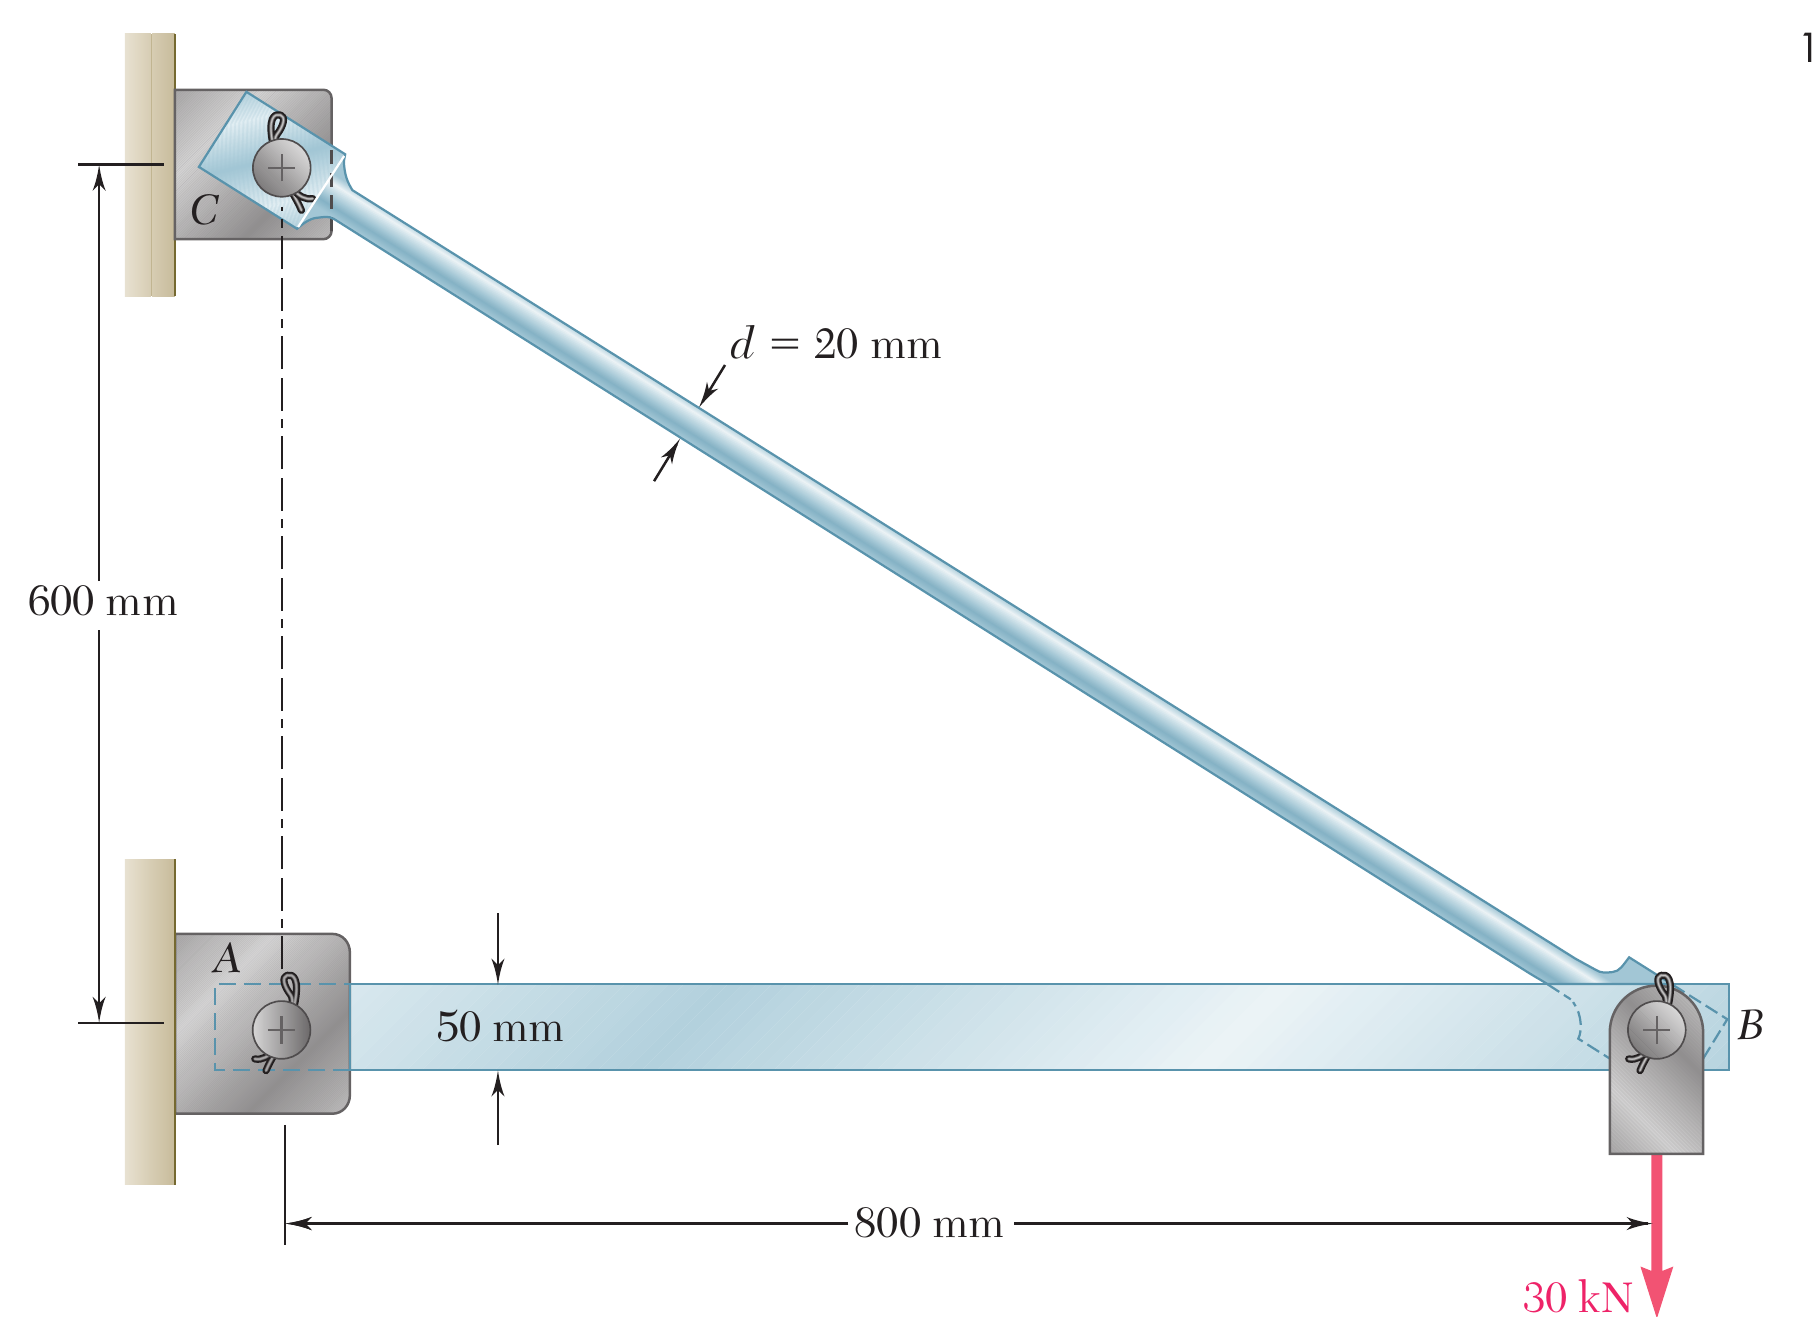
\includegraphics[width=\linewidth,height=5cm,keepaspectratio]{Chap_1/fig_1_1.png}
    \column{0.65\textwidth}
      \footnotesize
      \begin{itemize}
        \setlength{\itemsep}{0.5em}
        \item Thiết kế kết cấu mới đòi hỏi phải chọn vật liệu và kích
              thước cấu kiện phù hợp để đáp ứng các yêu cầu làm việc.
        \item Dựa trên các yếu tố về chi phí, trọng lượng, khả năng
              cung ứng, v.v., người ta chọn chế tạo thanh giằng bằng
              nhôm ($\sigma_{\mathrm{all}} = 100\,\mathrm{MPa}$).
              Hãy chọn đường kính thanh giằng phù hợp?
        \[
          \sigma_{\mathrm{all}} = \frac{P}{A}
          \quad\Rightarrow\quad
          A = \frac{P}{\sigma_{\mathrm{all}}}
            = \frac{50 \times 10^{3}\,\mathrm{N}}{100 \times 10^{6}\,\mathrm{Pa}}
            = 500 \times 10^{-6}\,\mathrm{m}^2
        \]
        \[
          A = \pi\frac{d^2}{4}
          \quad\Rightarrow\quad
        \]
        \[
          d = \sqrt{\frac{4A}{\pi}}
            = \sqrt{\frac{4\,(500 \times 10^{-6}\,\mathrm{m}^2)}{\pi}}
            = 2{,}52 \times 10^{-2}\,\mathrm{m} = 25{,}2\,\mathrm{mm}
        \]
        \item Thanh giằng bằng nhôm có đường kính từ 26 mm trở lên là
              đạt yêu cầu.
      \end{itemize}
  \end{columns}
\end{frame}
% ===========
\section{Lực dọc trục: ứng suất pháp}
\begin{frame}[t]{Lực dọc trục: ứng suất pháp}
  \begin{columns}[T]
    \column{0.38\textwidth}
      \centering
      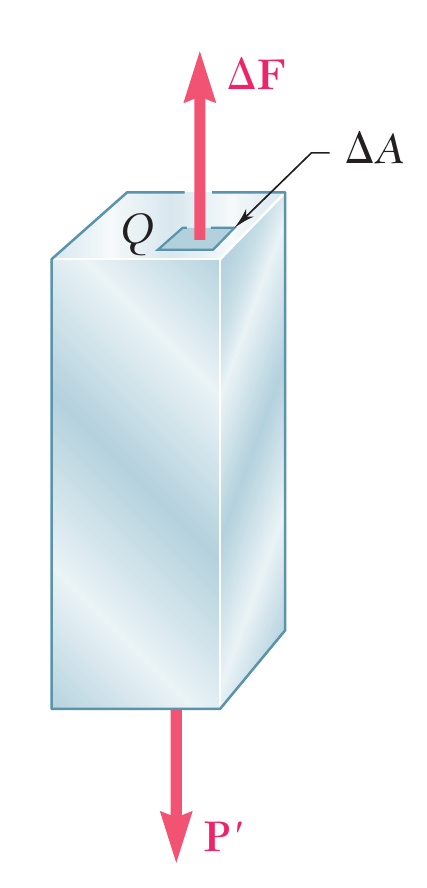
\includegraphics[width=\linewidth,height=2.9cm,keepaspectratio]{Chap_1/fig_1_9.png}\\[2pt]
      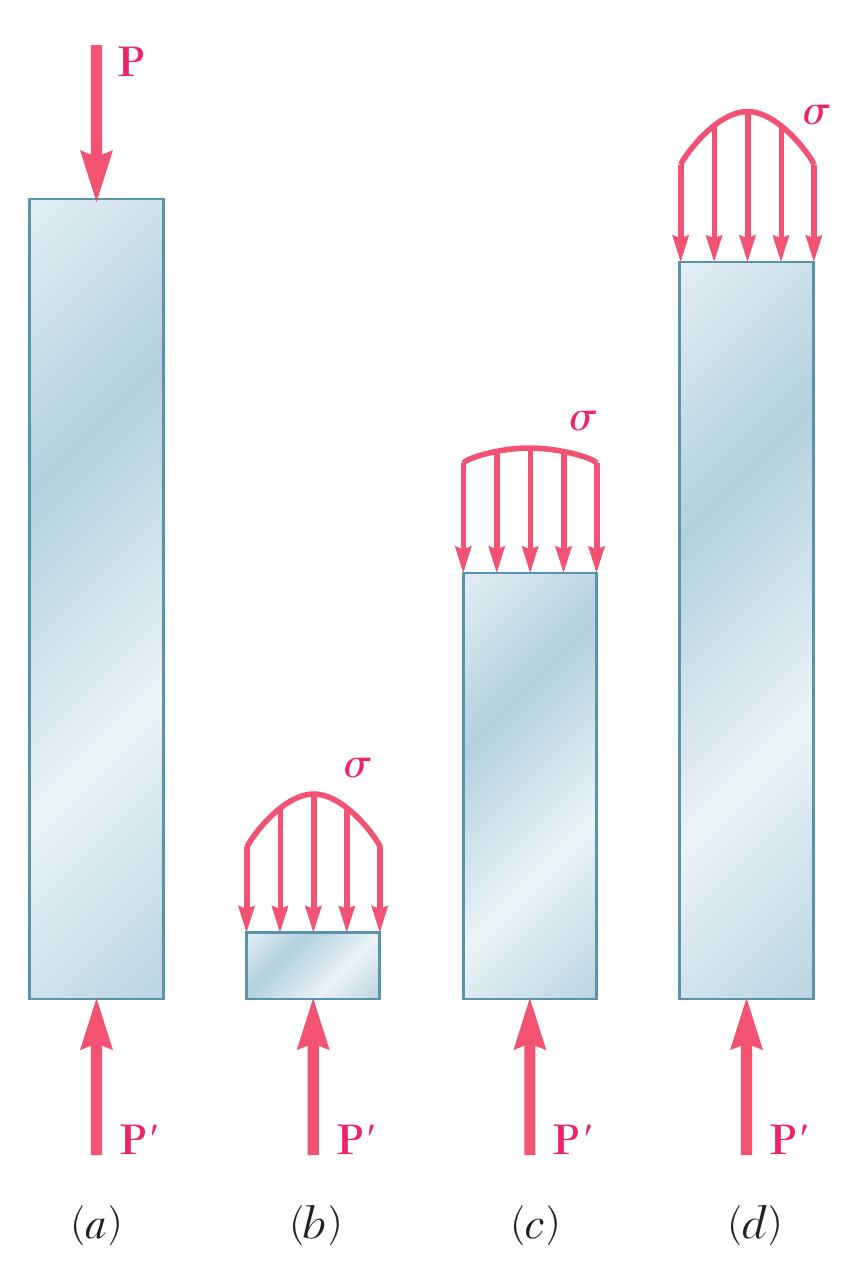
\includegraphics[width=\linewidth,height=3.5cm,keepaspectratio]{Chap_1/fig_1_10.png}
    \column{0.60\textwidth}
      \footnotesize
      \begin{itemize}
        \setlength{\itemsep}{0.5em}
        \item Hợp lực của các nội lực trong một cấu kiện chịu lực dọc
              trục có phương \emph{vuông góc} với mặt cắt ngang vuông
              góc với trục của cấu kiện.
        \item Cường độ lực trên mặt cắt đó được định nghĩa là ứng suất
              pháp.
        \[
          \sigma = \lim_{\Delta A \to 0} \frac{\Delta F}{\Delta A}
          \qquad
          \sigma_{\mathrm{tb}} = \frac{P}{A}
        \]
        \item Ứng suất pháp tại một điểm có thể không bằng ứng suất
              trung bình, nhưng hợp lực của phân bố ứng suất phải thỏa
              mãn:
        \[
          P = \sigma_{\mathrm{tb}} A = \int \mathrm{d}F
            = \int_A \sigma \,\mathrm{d}A
        \]
        \item Phân bố chi tiết của ứng suất là bài toán siêu tĩnh, tức
              là không thể xác định chỉ bằng các phương trình tĩnh học.
      \end{itemize}
  \end{columns}
\end{frame}
% ===========
\section{Tải trọng đúng tâm và lệch tâm}
\begin{frame}[t]{Tải trọng đúng tâm và lệch tâm}
  \begin{columns}[T]
    \column{0.38\textwidth}
      \centering
      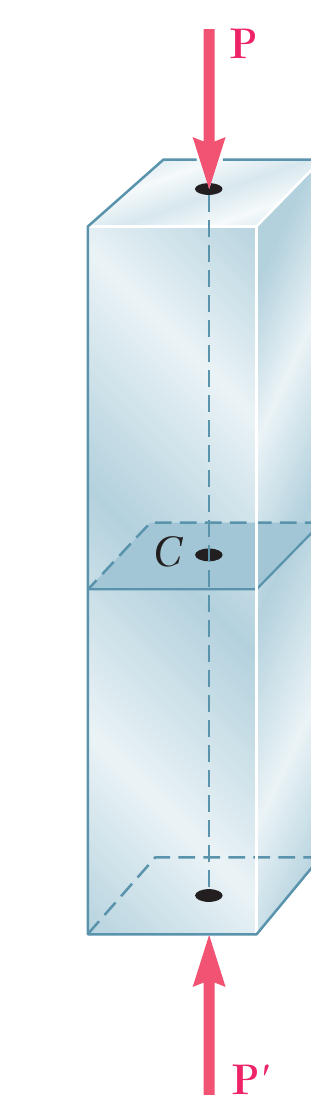
\includegraphics[width=\linewidth,height=2.9cm,keepaspectratio]{Chap_1/fig_1_12.png}\\[2pt]
      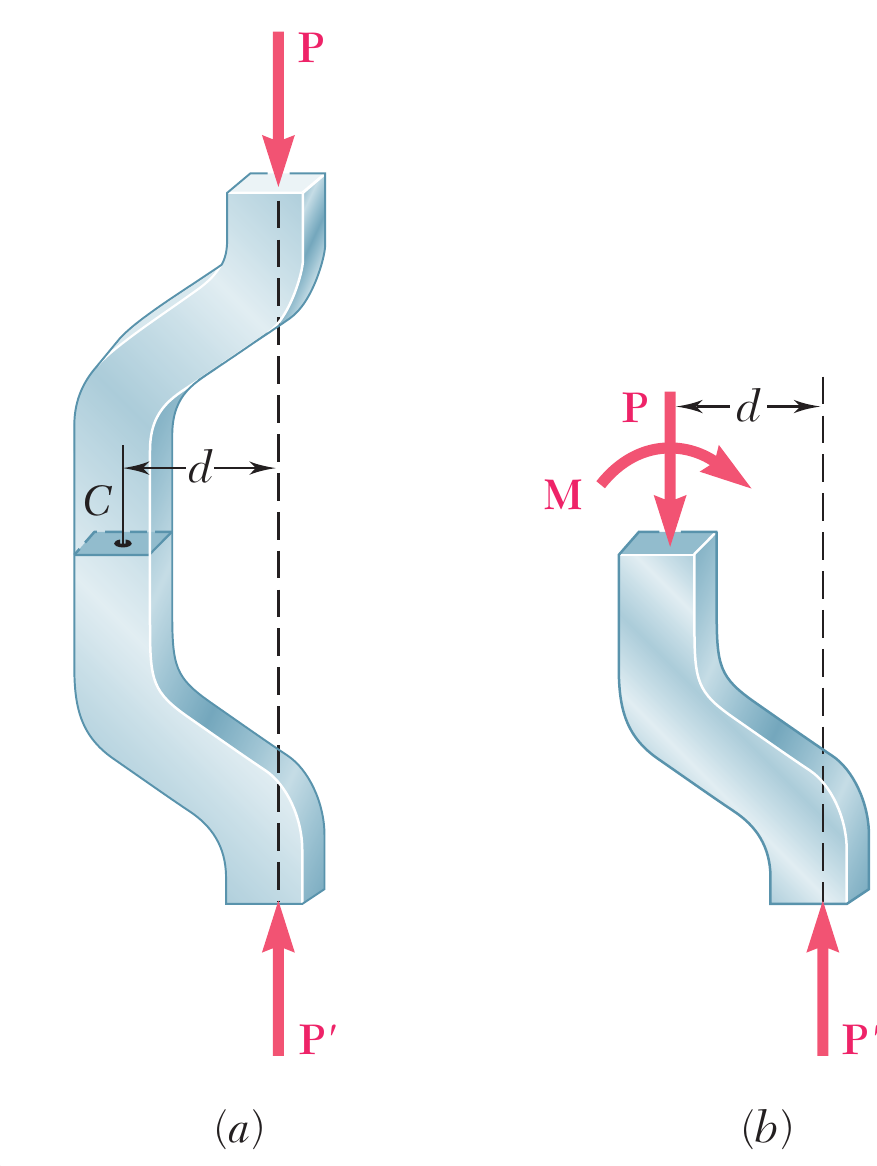
\includegraphics[width=\linewidth,height=3.5cm,keepaspectratio]{Chap_1/fig_1_13.png}
    \column{0.60\textwidth}
      \small
      \begin{itemize}
        \setlength{\itemsep}{0.7em}
        \item Ứng suất phân bố đều trên mặt cắt cho thấy đường tác dụng
              của hợp lực các nội lực đi qua trọng tâm của mặt cắt.
        \item Ứng suất chỉ có thể phân bố đều khi các lực tập trung đặt ở
              hai đầu của cấu kiện chịu hai lực đi qua trọng tâm mặt cắt.
              Trường hợp này được gọi là \emph{tải trọng đúng tâm}.
        \item Nếu cấu kiện chịu hai lực bị đặt tải \emph{lệch tâm}, thì
              hợp lực của phân bố ứng suất trên mặt cắt phải tạo ra một
              lực dọc trục và một mô men.
        \item Phân bố ứng suất trong cấu kiện chịu tải lệch tâm không thể
              đều hoặc đối xứng.
      \end{itemize}
  \end{columns}
\end{frame}
% ===========
\section{Ứng suất tiếp}
\begin{frame}[t]{Ứng suất tiếp}
  \begin{columns}[T]
    \column{0.38\textwidth}
      \centering
      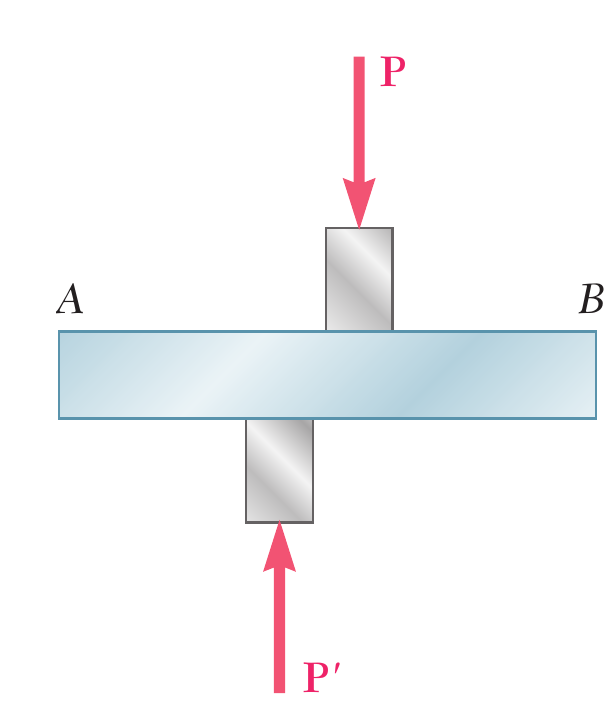
\includegraphics[width=\linewidth,height=3.5cm,keepaspectratio]{Chap_1/fig_1_14.png}\\[2pt]
      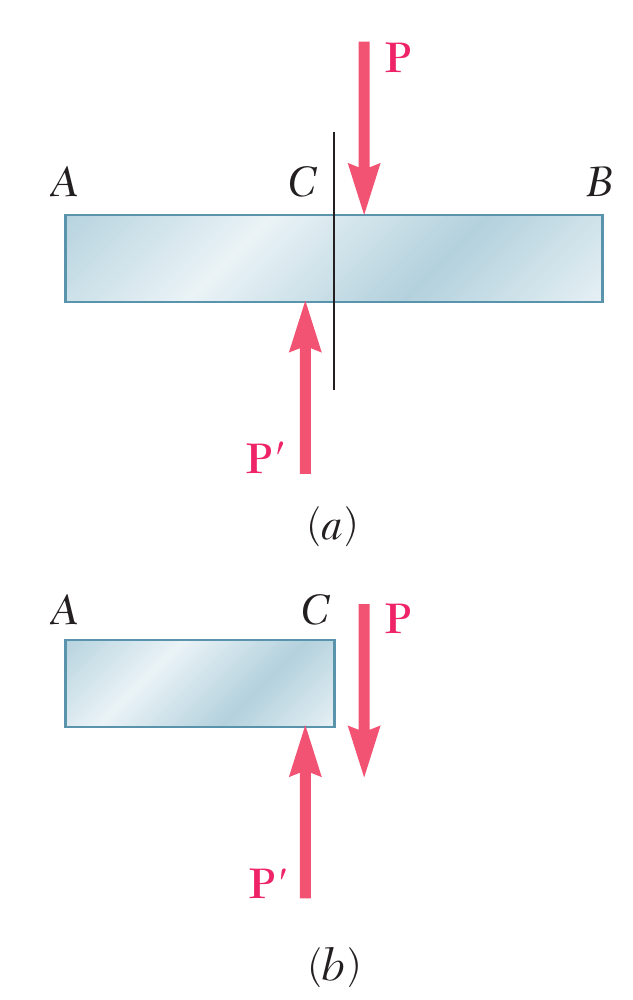
\includegraphics[width=\linewidth,height=3.5cm,keepaspectratio]{Chap_1/fig_1_15.png}
    \column{0.60\textwidth}
      \small
      \begin{itemize}
        \setlength{\itemsep}{0.3em}
        \item Các lực $P$ và $P'$ tác dụng theo phương ngang (vuông góc
              với trục) lên cấu kiện $AB$.
        \item Các nội lực tương ứng nằm trong mặt phẳng của mặt cắt $C$
              và được gọi là \emph{lực cắt}.
        \item Hợp lực của phân bố nội lực cắt được gọi là lực cắt của
              mặt cắt và bằng tải trọng $P$.
        \item Ứng suất tiếp trung bình tương ứng là:
              $\displaystyle \tau_{\mathrm{tb}} = \frac{P}{A}$
        \item Ứng suất tiếp thay đổi từ 0 tại bề mặt cấu kiện đến giá
              trị lớn nhất, có thể lớn hơn nhiều so với giá trị trung bình.
        \item Không thể giả thiết ứng suất tiếp phân bố đều.
      \end{itemize}
  \end{columns}
\end{frame}
% ===========
\section{Ví dụ về ứng suất tiếp}
\begin{frame}[t]{Ví dụ về ứng suất tiếp}
  \begin{columns}[T]
    \column{0.49\textwidth}
      \centering
      \textbf{Cắt đơn}\\[0.3em]
      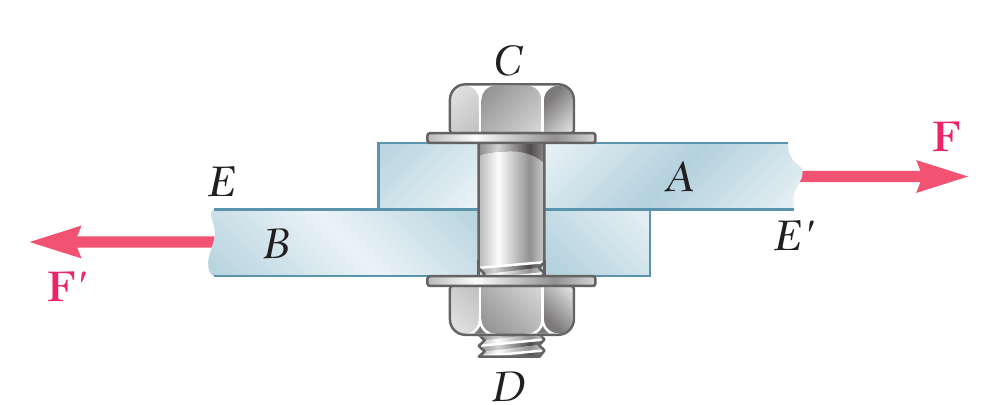
\includegraphics[width=0.9\linewidth,height=2.5cm,keepaspectratio]{Chap_1/fig_1_16.png}\\[2pt]
      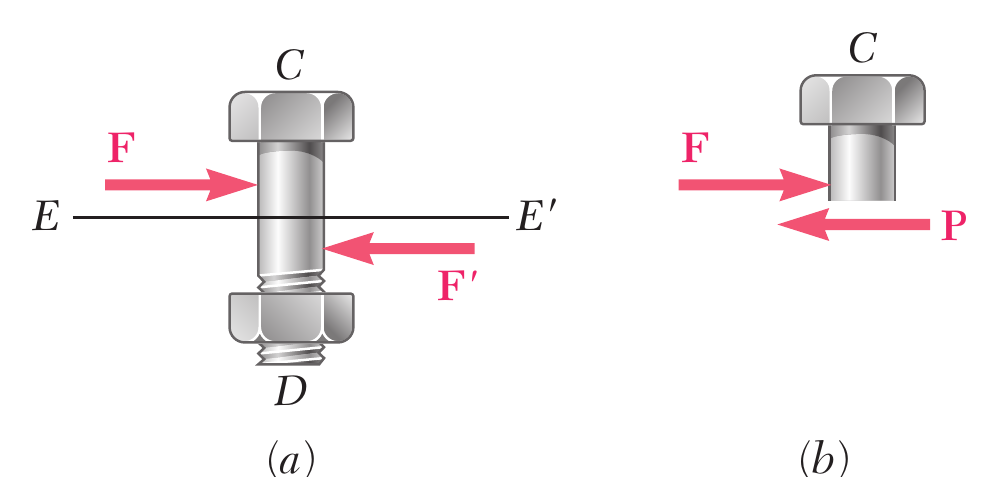
\includegraphics[width=0.9\linewidth,height=2.5cm,keepaspectratio]{Chap_1/fig_1_17.png}
      \[
        \tau_{\mathrm{tb}} = \frac{P}{A} = \frac{F}{A}
      \]
    \column{0.49\textwidth}
      \centering
      \textbf{Cắt đôi}\\[0.3em]
      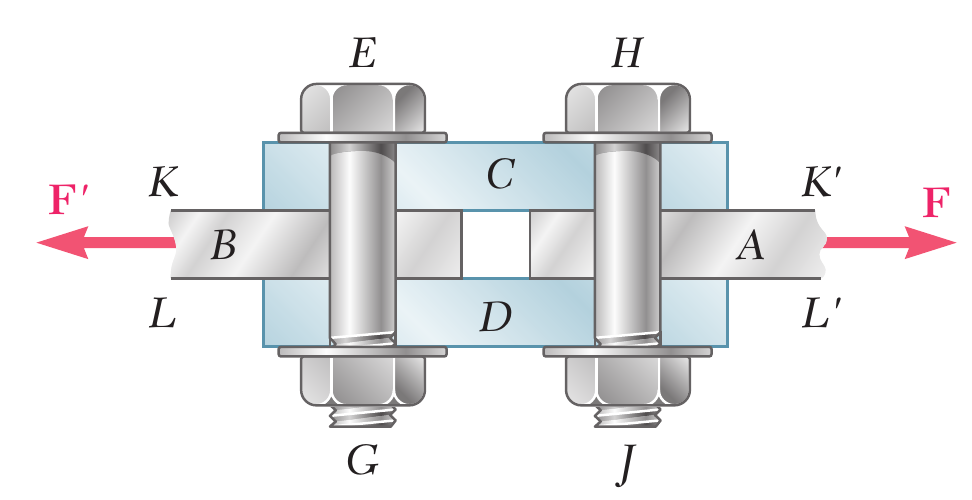
\includegraphics[width=0.9\linewidth,height=2.5cm,keepaspectratio]{Chap_1/fig_1_18.png}\\[2pt]
      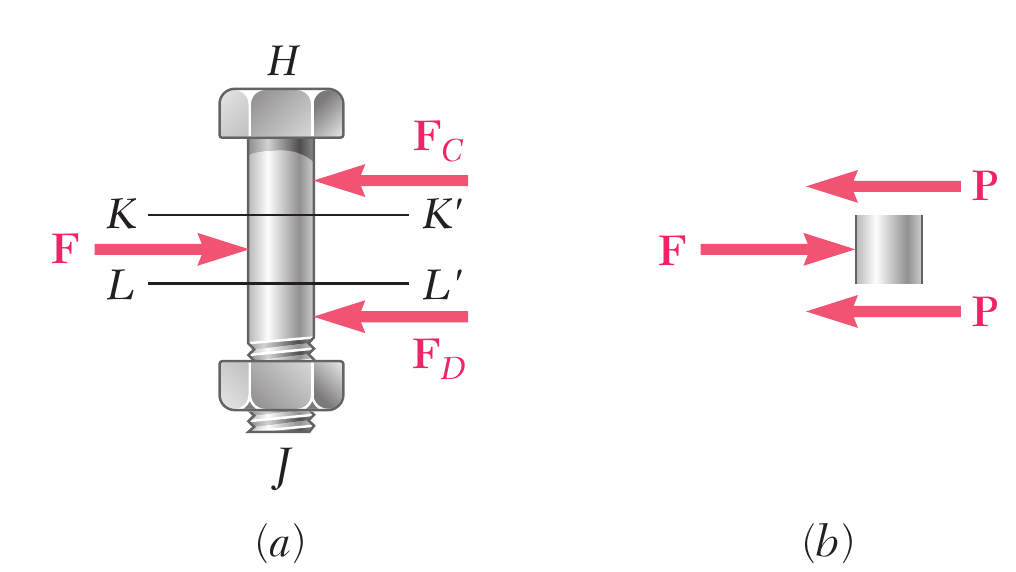
\includegraphics[width=0.9\linewidth,height=2.5cm,keepaspectratio]{Chap_1/fig_1_19.png}
      \[
        \tau_{\mathrm{tb}} = \frac{P}{A} = \frac{F}{2A}
      \]
  \end{columns}
\end{frame}
% ===========
\section{Ứng suất dập trong mối ghép}
\begin{frame}[t]{Ứng suất dập trong mối ghép}
  \begin{columns}[T]
    \column{0.42\textwidth}
      \centering
      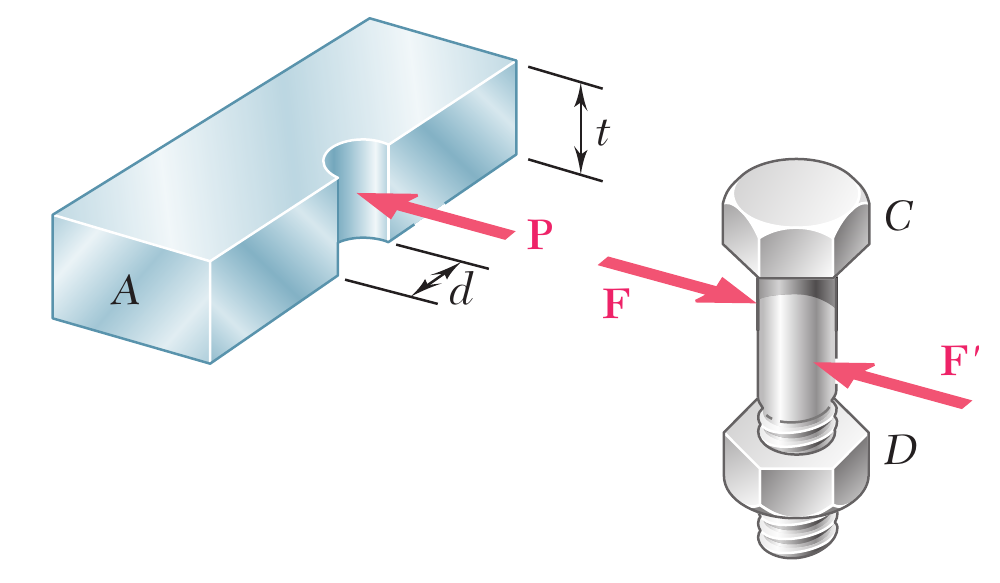
\includegraphics[width=\linewidth,height=2.9cm,keepaspectratio]{Chap_1/fig_1_20.png}\\[2pt]
      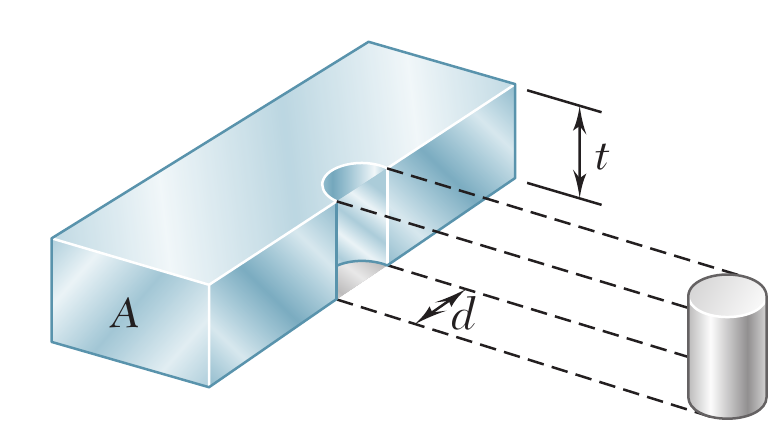
\includegraphics[width=\linewidth,height=2.9cm,keepaspectratio]{Chap_1/fig_1_21.png}
    \column{0.56\textwidth}
      \small
      \begin{itemize}
        \setlength{\itemsep}{0.8em}
        \item Bu lông, đinh tán và chốt gây ra ứng suất tại các điểm
              tiếp xúc, hay các bề mặt tựa (bề mặt dập), của các cấu kiện
              mà chúng liên kết.
        \item Hợp lực của phân bố lực trên bề mặt bằng và ngược chiều
              với lực tác dụng lên chốt.
        \item Cường độ lực trung bình tương ứng được gọi là \emph{ứng
              suất dập}:
        \[
          \sigma_b = \frac{P}{A} = \frac{P}{t\,d}
        \]
      \end{itemize}
  \end{columns}
\end{frame}
% ===========
\section{Ví dụ phân tích ứng suất và thiết kế}
\begin{frame}[t]{Ví dụ phân tích ứng suất và thiết kế}
  \begin{columns}[T]
    \column{0.48\textwidth}
      \centering
      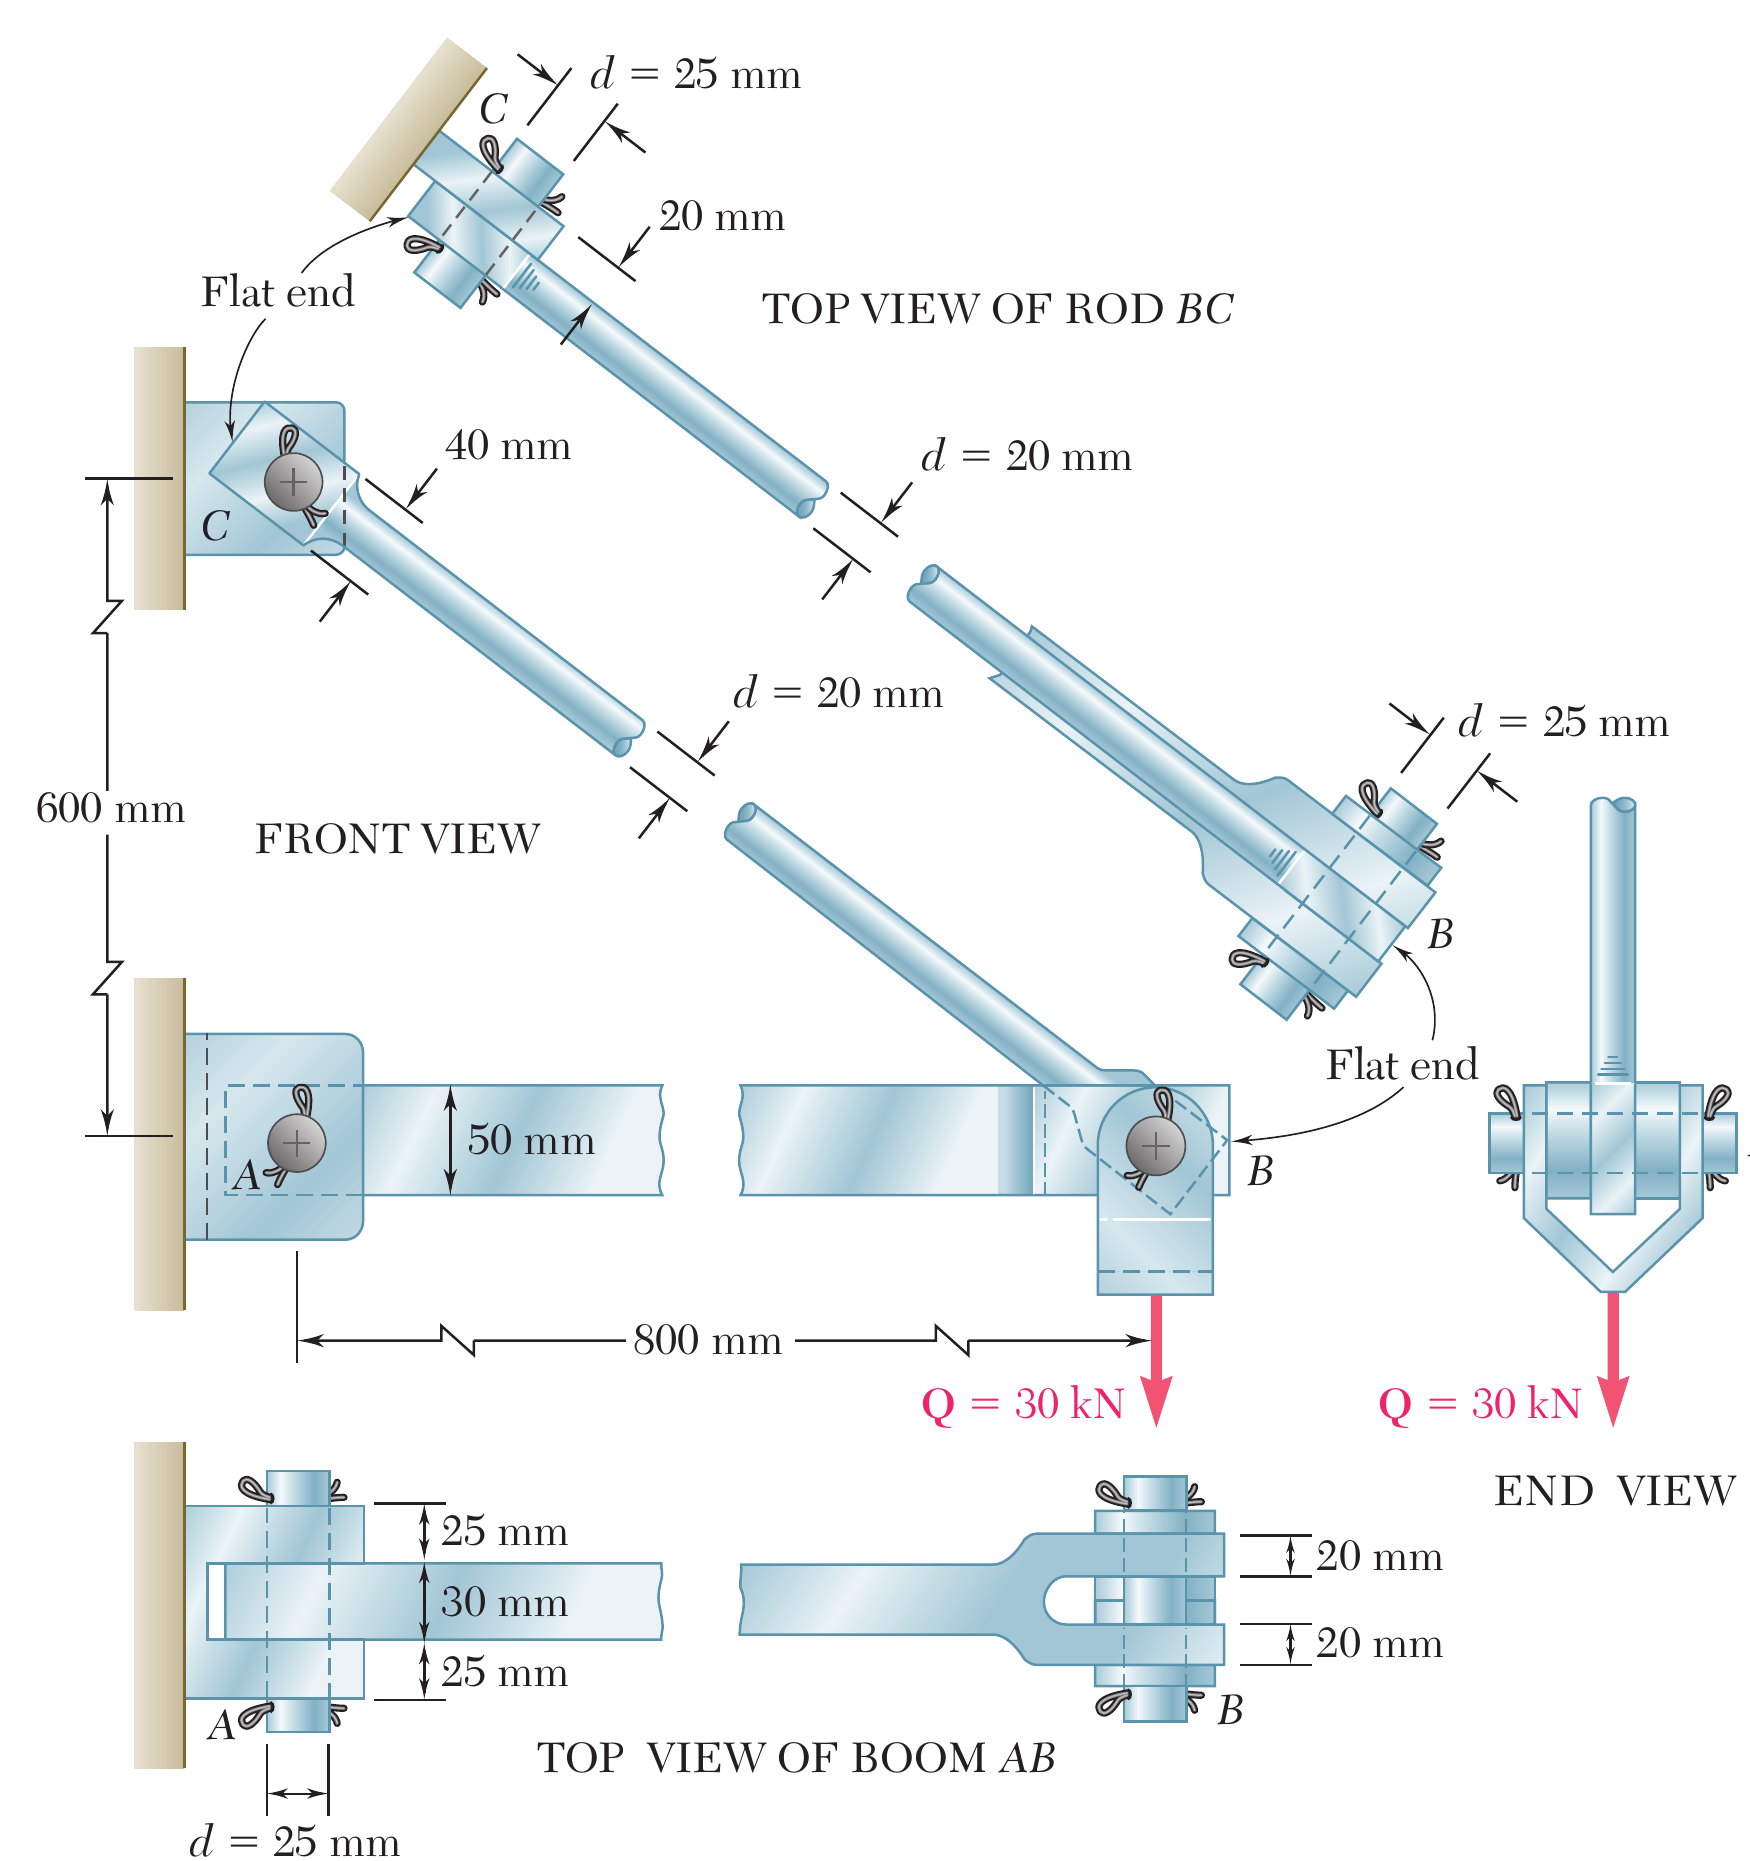
\includegraphics[width=\linewidth,height=6cm,keepaspectratio]{Chap_1/fig_1_22.png}
    \column{0.50\textwidth}
      \small
      \begin{itemize}
        \setlength{\itemsep}{0.8em}
        \item Cần xác định ứng suất trong các cấu kiện và các mối ghép
              của kết cấu như hình vẽ.
        \item Từ phân tích tĩnh học:
        \[
          F_{AB} = 40\,\mathrm{kN}\ \text{(nén)}, \qquad
          F_{BC} = 50\,\mathrm{kN}\ \text{(kéo)}
        \]
        \item Cần xét ứng suất pháp lớn nhất trong $AB$ và $BC$, ứng
              suất tiếp và ứng suất dập tại mỗi liên kết chốt.
      \end{itemize}
  \end{columns}
\end{frame}
% ===========
\section{Ứng suất pháp trong thanh giằng và dầm}
\begin{frame}[t]{Ứng suất pháp trong thanh giằng và dầm}
  \begin{columns}[T]
    \column{0.36\textwidth}
      \centering
      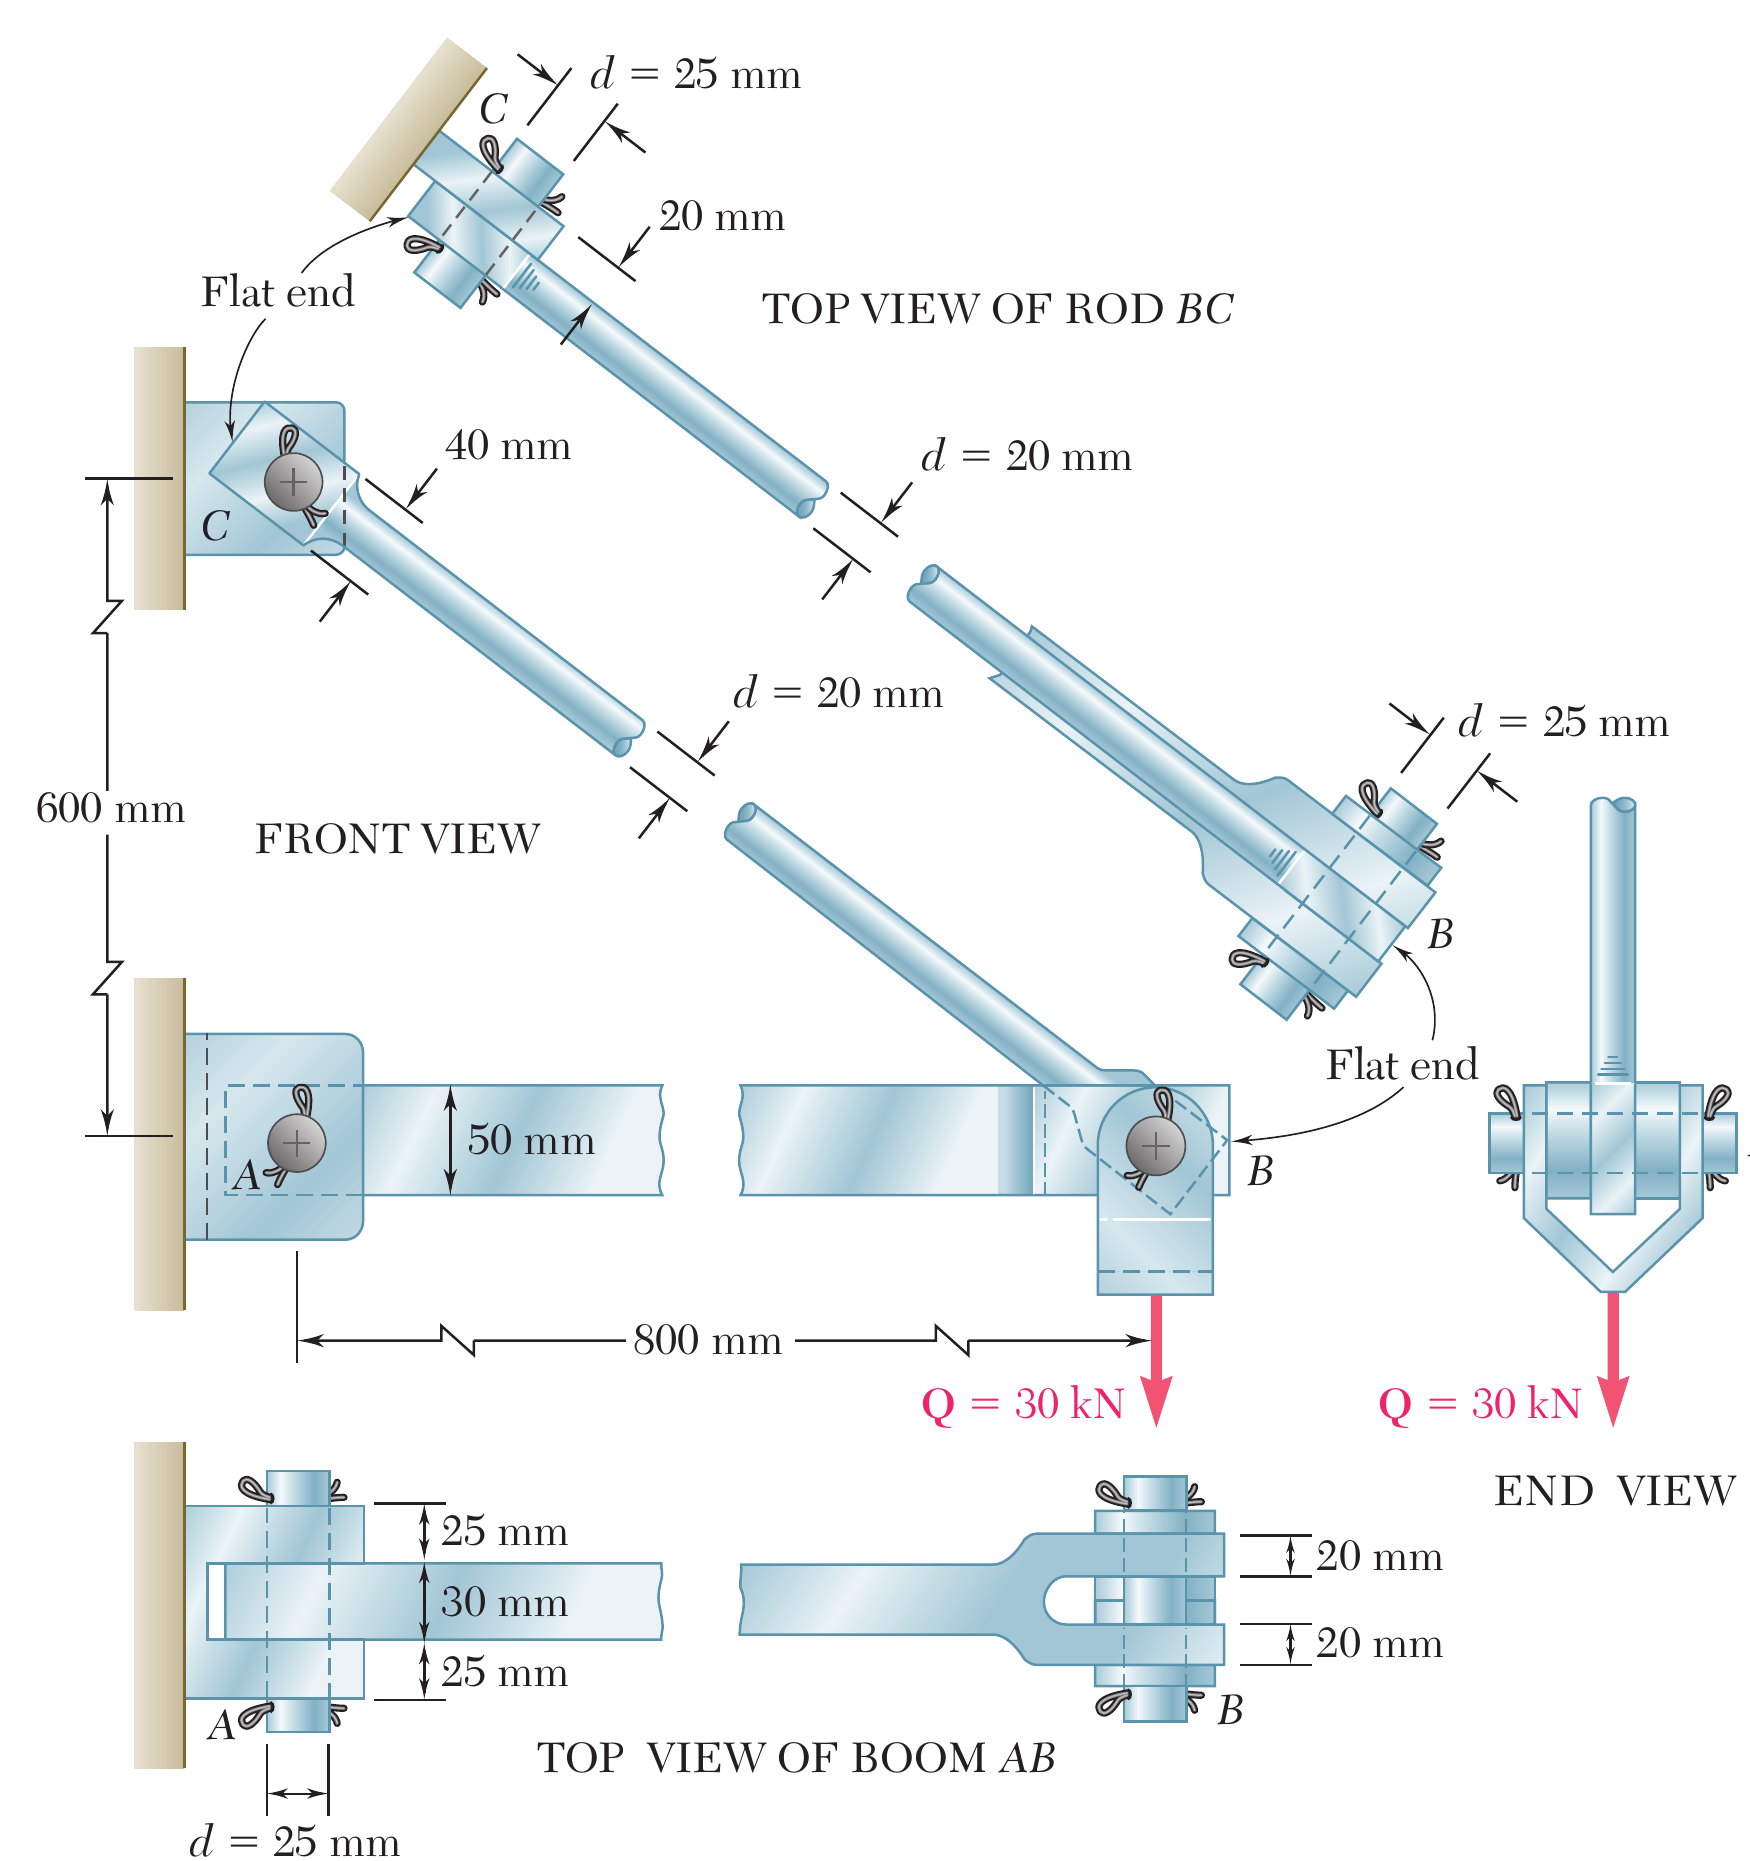
\includegraphics[width=\linewidth,height=5.5cm,keepaspectratio]{Chap_1/fig_1_22.png}
    \column{0.62\textwidth}
      \footnotesize
      \begin{itemize}
        \setlength{\itemsep}{0.5em}
        \item Thanh giằng chịu kéo với lực dọc trục 50 kN.
        \item Tại phần giữa thanh, ứng suất pháp trung bình trên mặt cắt
              tròn ($A = 314\times10^{-6}\,\mathrm{m}^2$) là
              $\sigma_{BC} = +159\,\mathrm{MPa}$.
        \item Tại hai đầu dẹt của thanh, diện tích mặt cắt nhỏ nhất nằm
              trên đường tâm chốt:
        \[
          A = (20\,\mathrm{mm})(40\,\mathrm{mm} - 25\,\mathrm{mm})
            = 300\times10^{-6}\,\mathrm{m}^2
        \]
        \[
          \sigma_{BC,\mathrm{đầu}} = \frac{P}{A}
          = \frac{50\times10^{3}\,\mathrm{N}}{300\times10^{-6}\,\mathrm{m}^2}
          = 167\,\mathrm{MPa}
        \]
        \item Dầm chịu nén với lực dọc trục 40 kN và ứng suất pháp trung
              bình $-26{,}7\,\mathrm{MPa}$.
        \item Các mặt cắt có diện tích nhỏ nhất ở hai đầu dầm không chịu
              ứng suất do dầm chịu nén.
      \end{itemize}
  \end{columns}
\end{frame}
% ===========
\section{Ứng suất tiếp trong chốt}
\begin{frame}[t]{Ứng suất tiếp trong chốt}
  \begin{columns}[T]
    \column{0.36\textwidth}
      \centering
      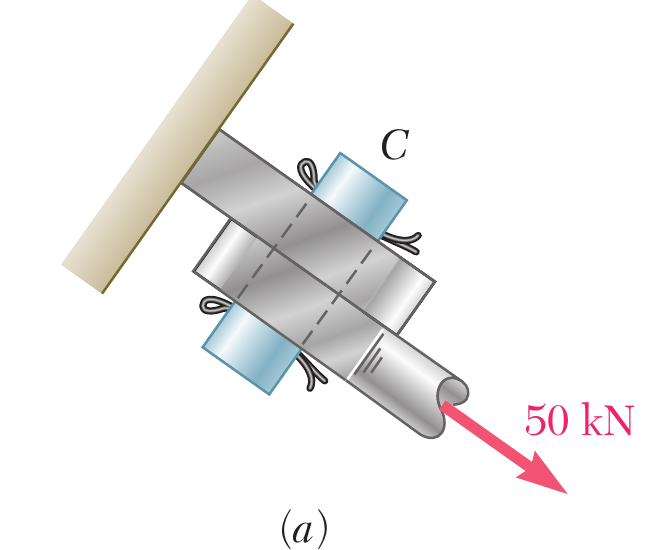
\includegraphics[width=\linewidth,height=1.5cm,keepaspectratio]{Chap_1/fig_1_23a.png}\\[2pt]
      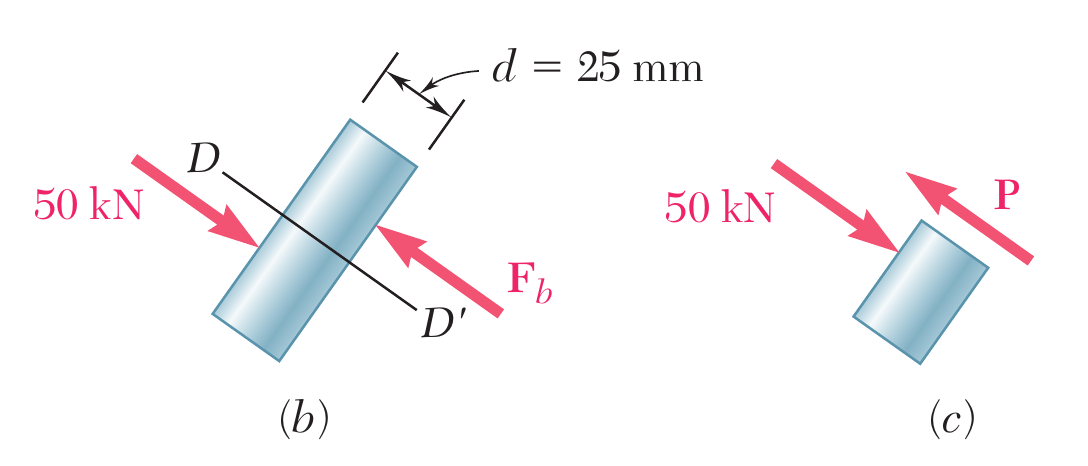
\includegraphics[width=\linewidth,height=1.5cm,keepaspectratio]{Chap_1/fig_1_23bc.png}\\[2pt]
      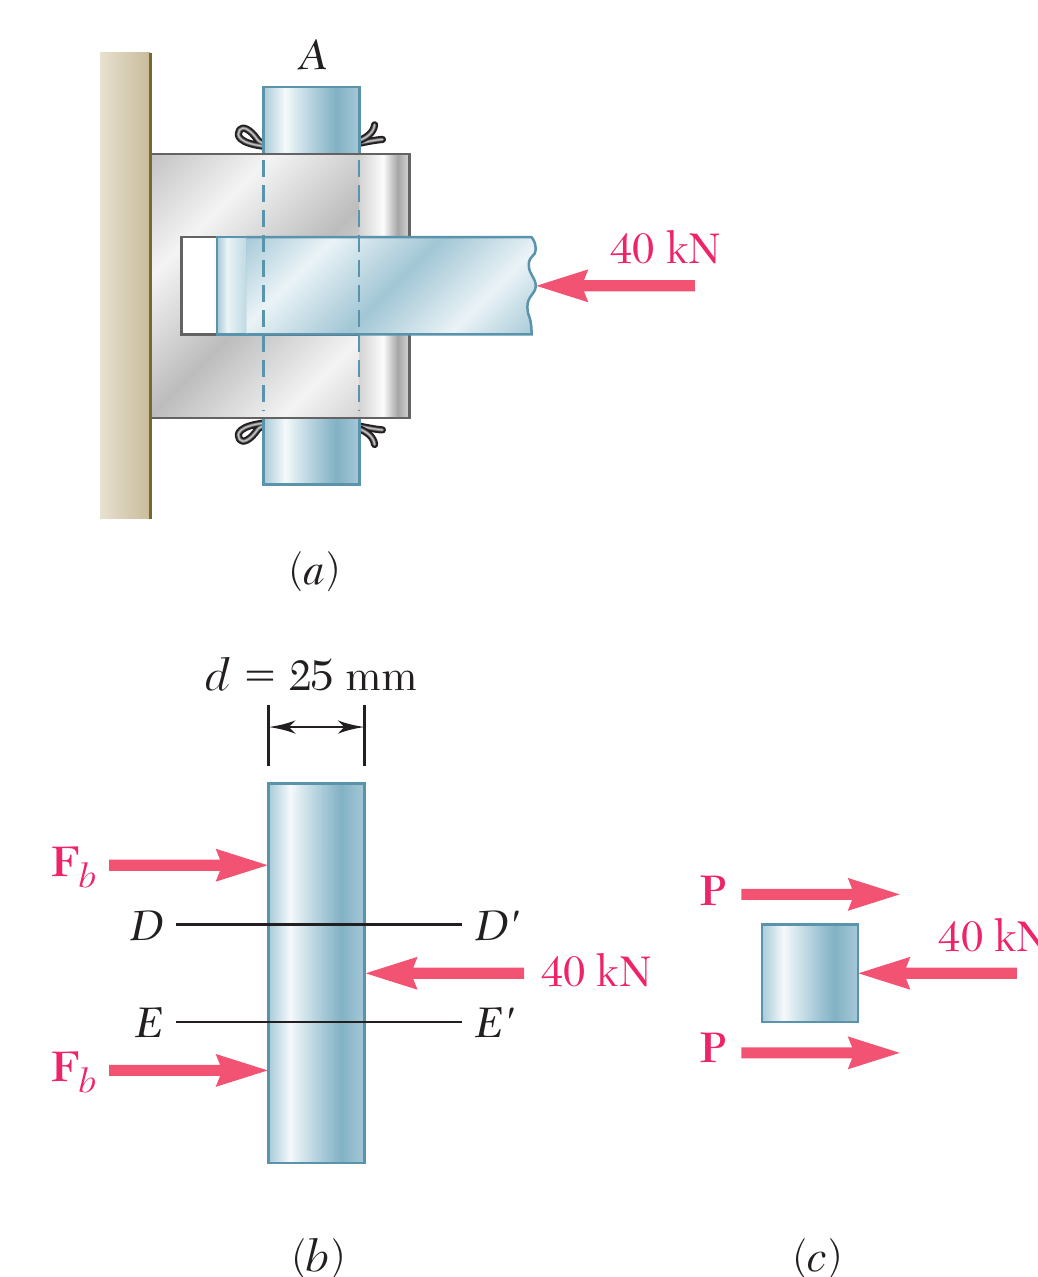
\includegraphics[width=\linewidth,height=4cm,keepaspectratio]{Chap_1/fig_1_24.png}
    \column{0.62\textwidth}
      \footnotesize
      \begin{itemize}
        \setlength{\itemsep}{0.4em}
        \item Diện tích mặt cắt ngang của các chốt tại $A$, $B$ và $C$:
        \[
          A = \pi r^2 = \pi\left(\frac{25\,\mathrm{mm}}{2}\right)^2
            = 491\times10^{-6}\,\mathrm{m}^2
        \]
        \item Lực tác dụng lên chốt tại $C$ bằng lực do thanh giằng $BC$
              tác dụng:
        \[
          \tau_{C,\mathrm{tb}} = \frac{P}{A}
          = \frac{50\times10^{3}\,\mathrm{N}}{491\times10^{-6}\,\mathrm{m}^2}
          = 102\,\mathrm{MPa}
        \]
        \item Chốt tại $A$ chịu cắt đôi với tổng lực bằng lực do dầm
              $AB$ tác dụng:
        \[
          \tau_{A,\mathrm{tb}} = \frac{P}{A}
          = \frac{20\,\mathrm{kN}}{491\times10^{-6}\,\mathrm{m}^2}
          = 40{,}7\,\mathrm{MPa}
        \]
      \end{itemize}
  \end{columns}
\end{frame}
% ===========
\begin{frame}[t]{Ứng suất tiếp trong chốt (tiếp)}
  \begin{columns}[T]
    \column{0.40\textwidth}
      \centering
      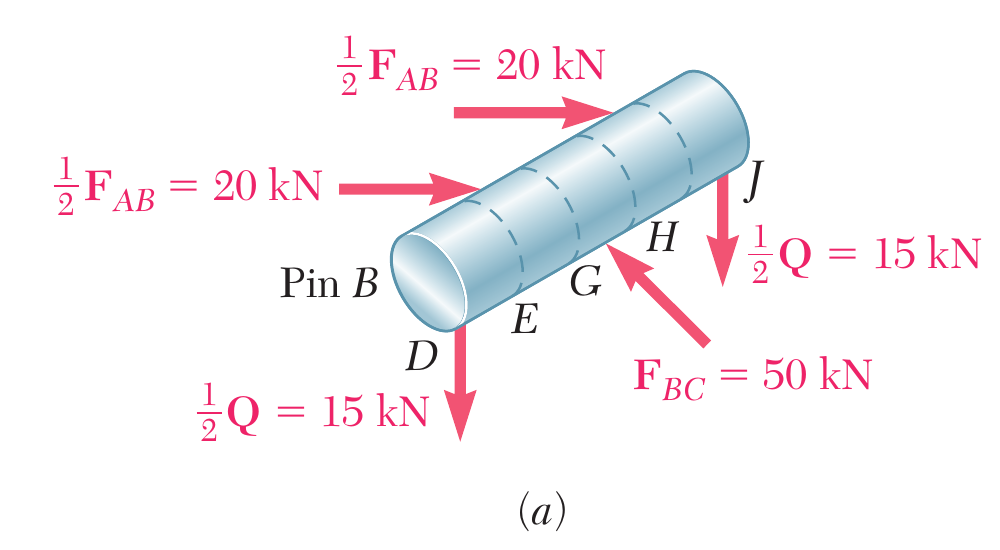
\includegraphics[width=\linewidth,height=2.5cm,keepaspectratio]{Chap_1/fig_1_25a.png}\\[2pt]
      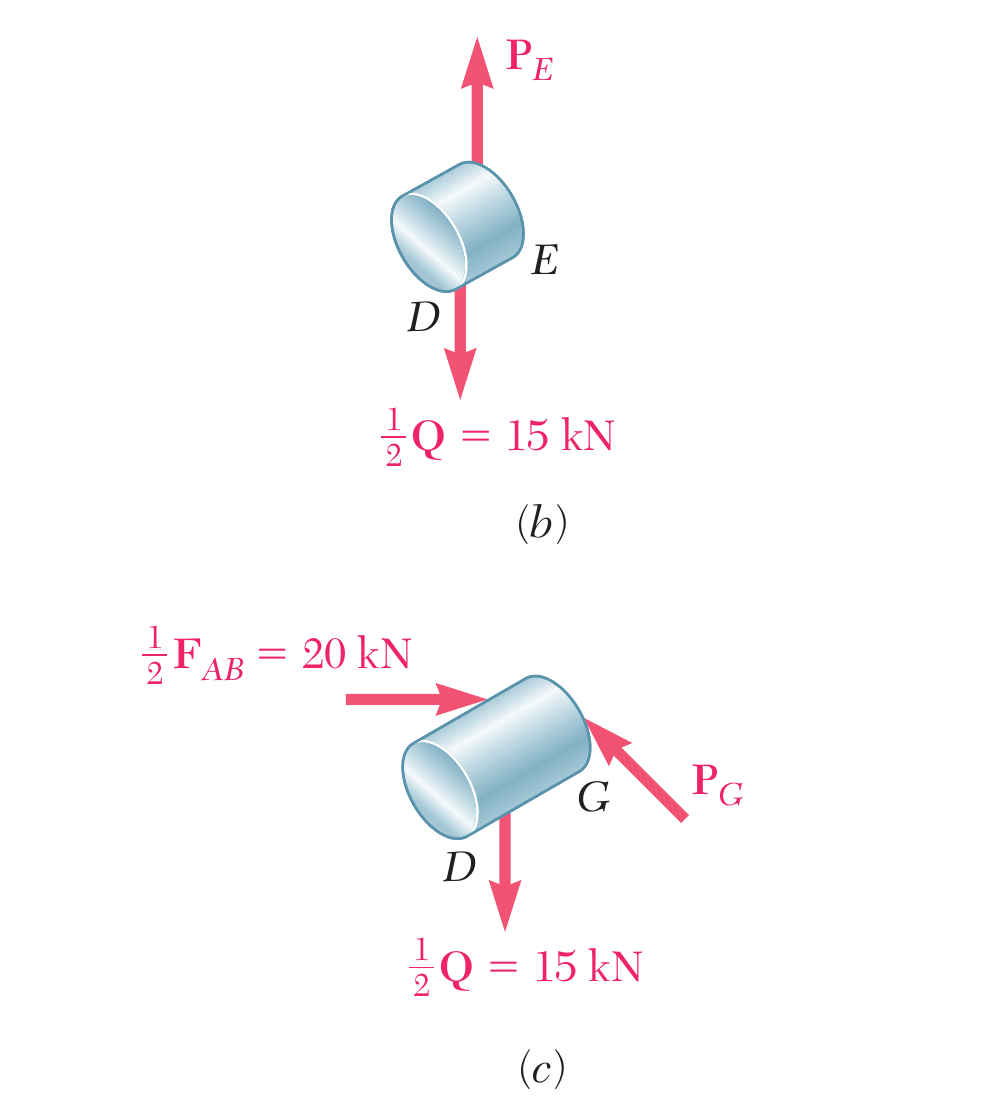
\includegraphics[width=\linewidth,height=4.5cm,keepaspectratio]{Chap_1/fig_1_25bc.png}
    \column{0.58\textwidth}
      \small
      \begin{itemize}
        \setlength{\itemsep}{0.8em}
        \item Chia chốt tại $B$ thành các đoạn để tìm mặt cắt có lực cắt
              lớn nhất:
        \[
          P_E = 15\,\mathrm{kN}, \qquad
          P_G = 25\,\mathrm{kN}\ \text{(lớn nhất)}
        \]
        \item Tính ứng suất tiếp trung bình tương ứng:
        \[
          \tau_{B,\mathrm{tb}} = \frac{P_G}{A}
          = \frac{25\,\mathrm{kN}}{491\times10^{-6}\,\mathrm{m}^2}
          = 50{,}9\,\mathrm{MPa}
        \]
      \end{itemize}
  \end{columns}
\end{frame}
% ===========
\section{Ứng suất dập tại chốt}
\begin{frame}[t]{Ứng suất dập tại chốt}
  \begin{columns}[T]
    \column{0.40\textwidth}
      \centering
      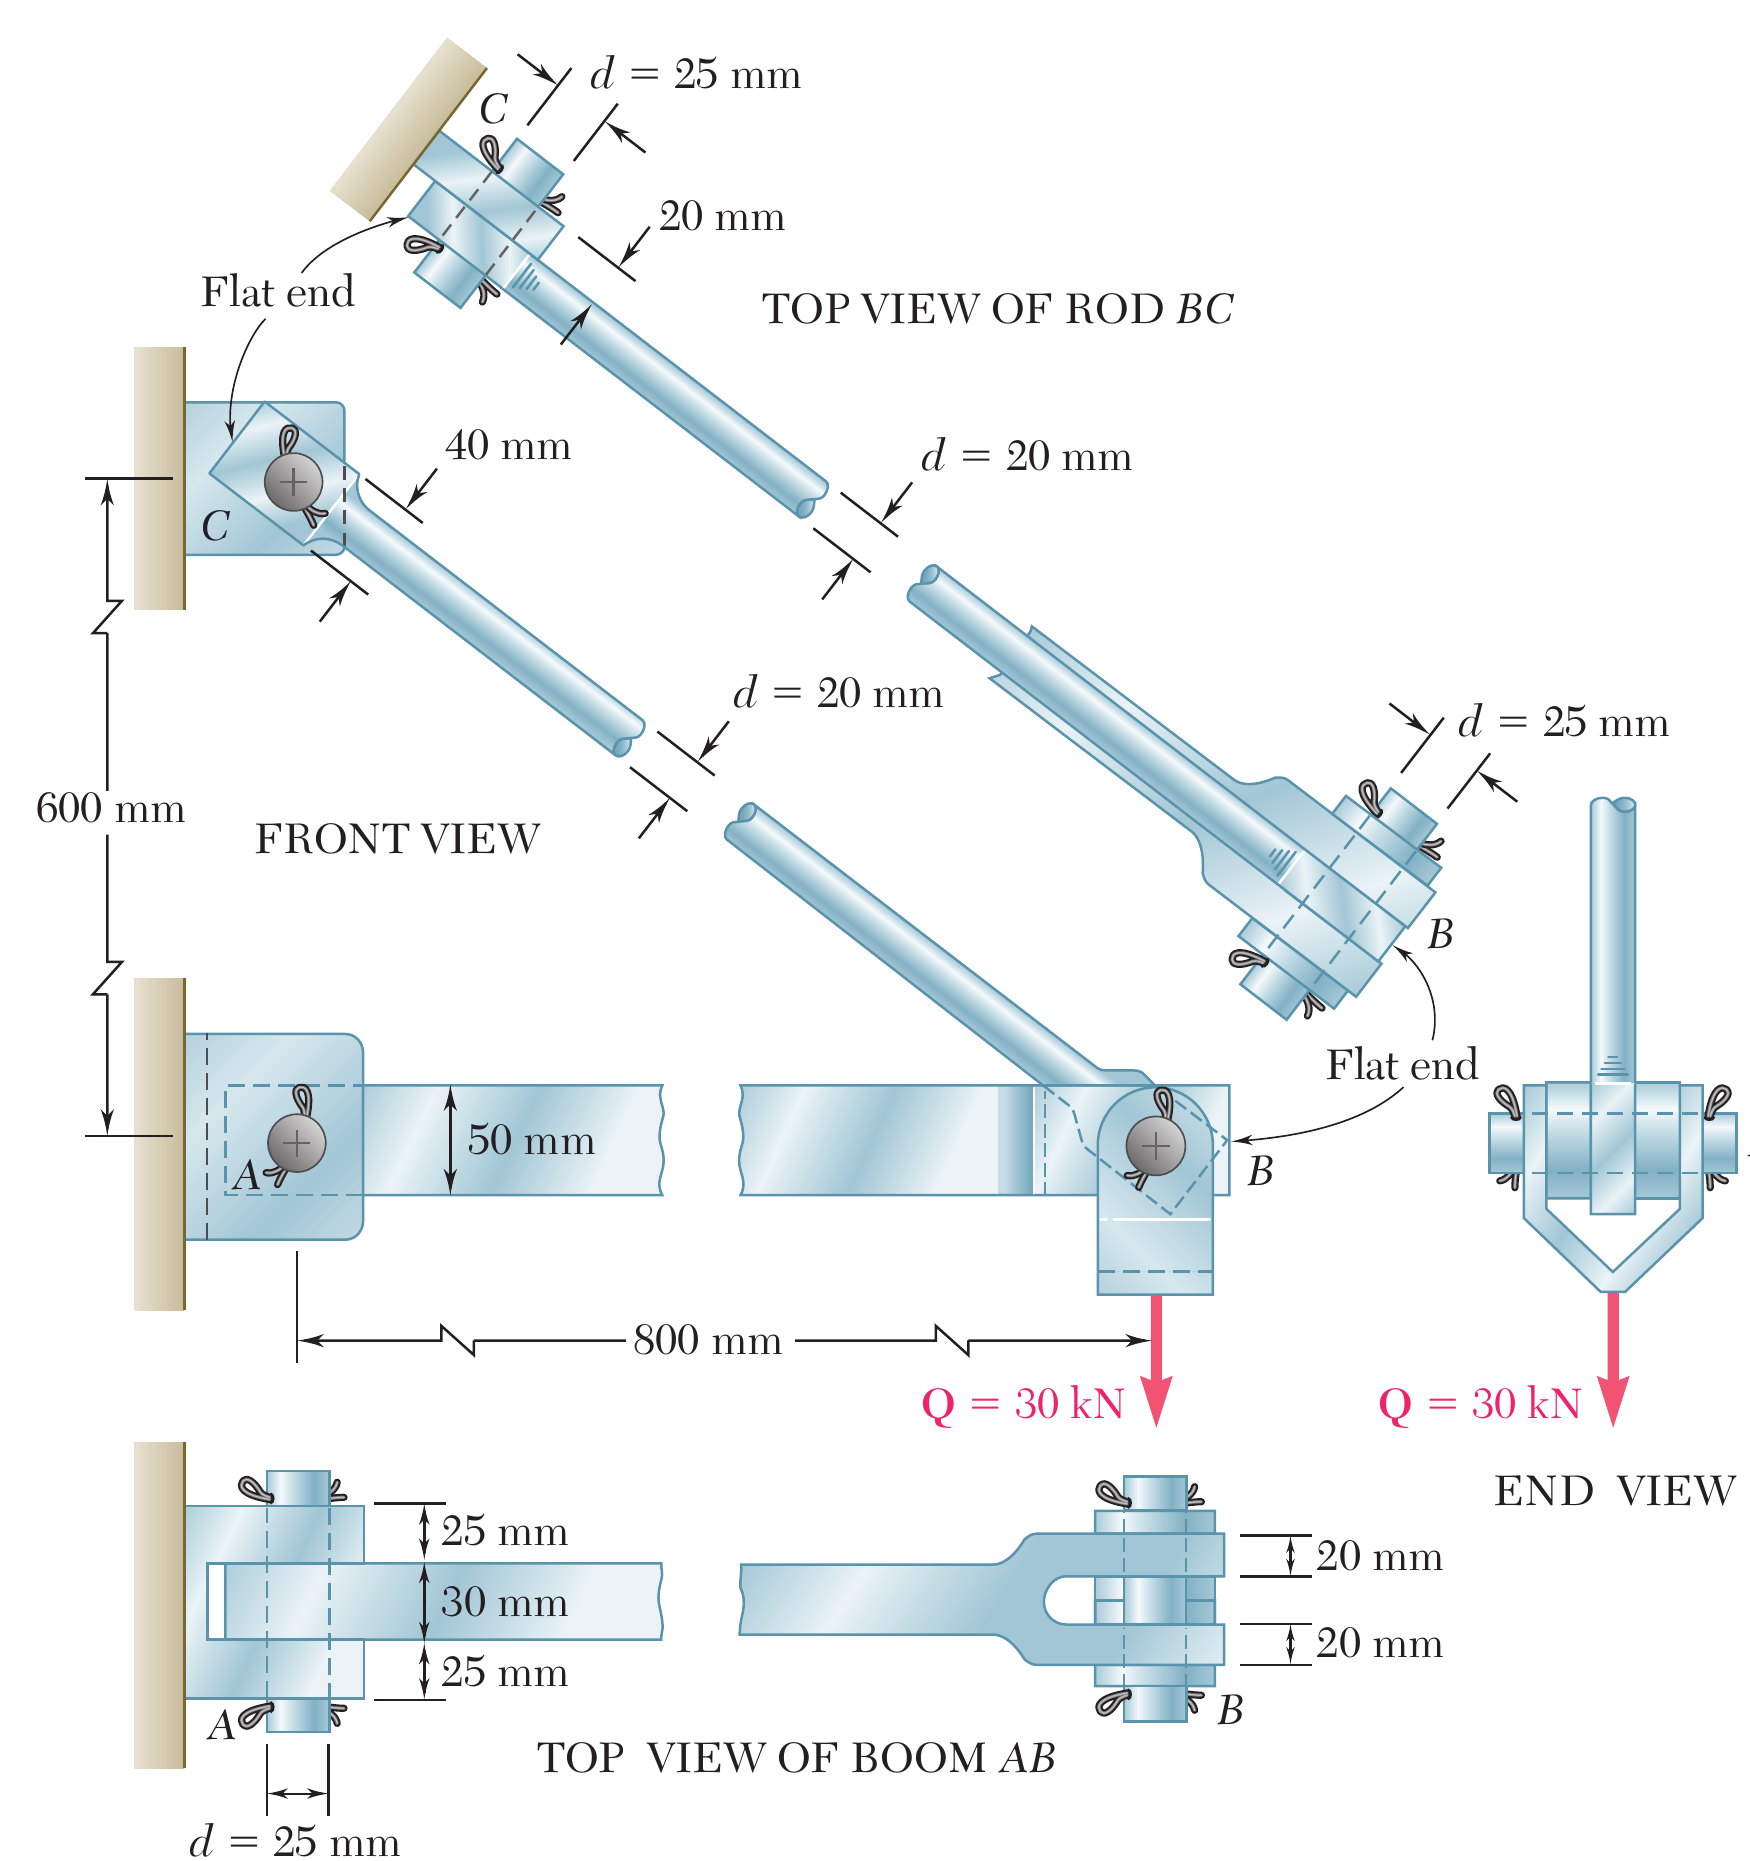
\includegraphics[width=\linewidth,height=5cm,keepaspectratio]{Chap_1/fig_1_22.png}
    \column{0.58\textwidth}
      \small
      \begin{itemize}
        \setlength{\itemsep}{0.8em}
        \item Để xác định ứng suất dập tại $A$ trên dầm $AB$, ta có
              $t = 30\,\mathrm{mm}$ và $d = 25\,\mathrm{mm}$:
        \[
          \sigma_b = \frac{P}{t\,d}
          = \frac{40\,\mathrm{kN}}{(30\,\mathrm{mm})(25\,\mathrm{mm})}
          = 53{,}3\,\mathrm{MPa}
        \]
        \item Để xác định ứng suất dập tại $A$ trên giá đỡ, ta có
              $t = 2(25\,\mathrm{mm}) = 50\,\mathrm{mm}$ và
              $d = 25\,\mathrm{mm}$:
        \[
          \sigma_b = \frac{P}{t\,d}
          = \frac{40\,\mathrm{kN}}{(50\,\mathrm{mm})(25\,\mathrm{mm})}
          = 32{,}0\,\mathrm{MPa}
        \]
      \end{itemize}
  \end{columns}
\end{frame}
% ===========
\section{Ứng suất trong cấu kiện chịu hai lực}
\begin{frame}[t]{Ứng suất trong cấu kiện chịu hai lực}
  \begin{columns}[T]
    \column{0.40\textwidth}
      \centering
      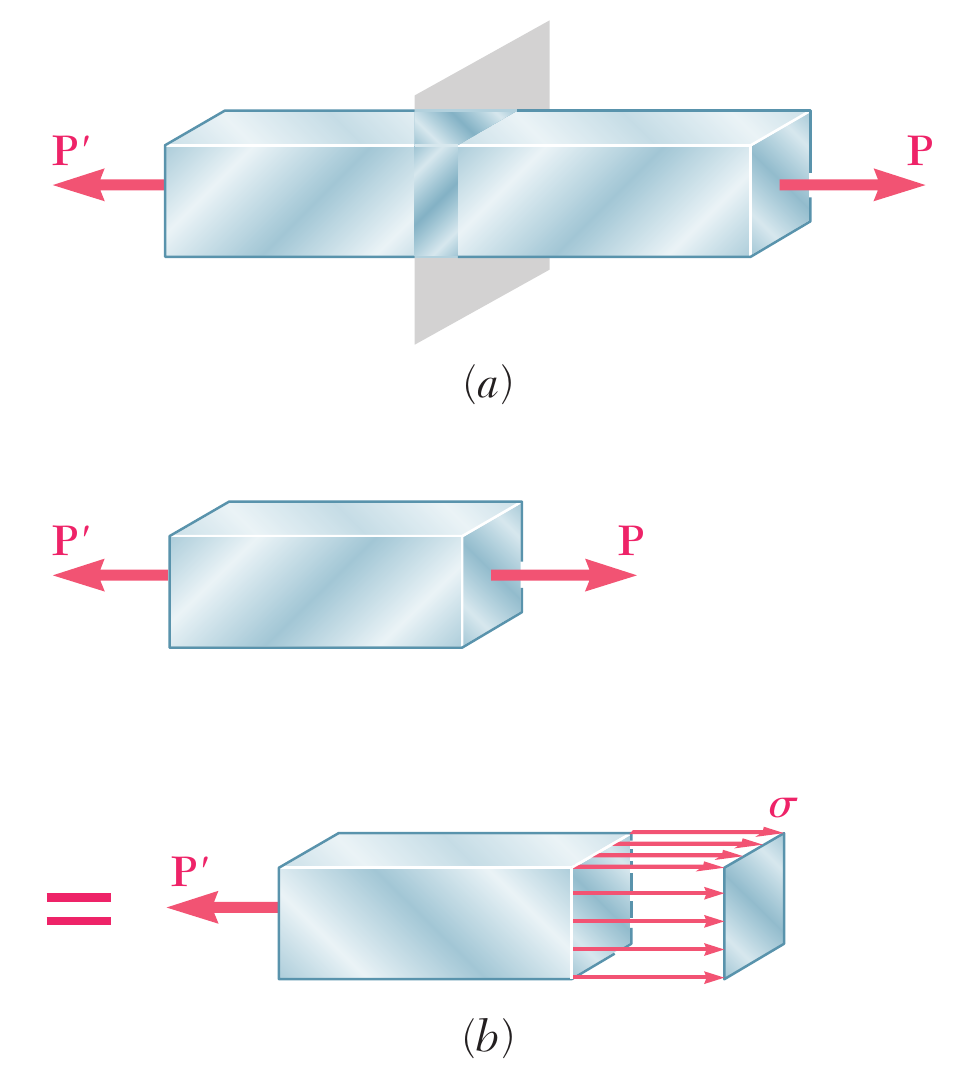
\includegraphics[width=\linewidth,height=4.5cm,keepaspectratio]{Chap_1/fig_1_26.png}\\[2pt]
      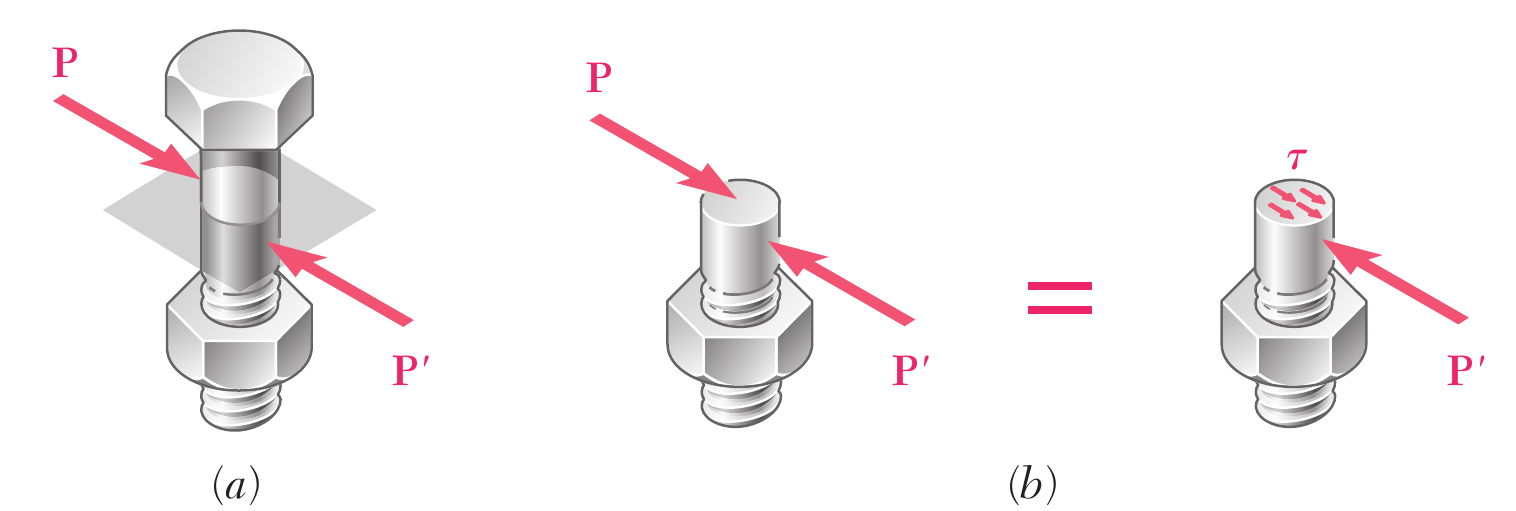
\includegraphics[width=\linewidth,height=4.5cm,keepaspectratio]{Chap_1/fig_1_27.png}
    \column{0.58\textwidth}
      \small
      \begin{itemize}
        \setlength{\itemsep}{0.9em}
        \item Lực dọc trục tác dụng lên cấu kiện chịu hai lực chỉ gây ra
              ứng suất pháp trên mặt cắt vuông góc với trục cấu kiện.
        \item Lực ngang tác dụng lên bu lông và chốt chỉ gây ra ứng suất
              tiếp trên mặt phẳng vuông góc với trục bu lông hoặc chốt.
        \item Ta sẽ chứng minh rằng lực dọc trục hoặc lực ngang đều có
              thể gây ra cả ứng suất pháp lẫn ứng suất tiếp trên một mặt
              phẳng không vuông góc với trục cấu kiện.
      \end{itemize}
  \end{columns}
\end{frame}
% ===========
\section{Ứng suất trên mặt cắt nghiêng}
\begin{frame}[t]{Ứng suất trên mặt cắt nghiêng}
  \begin{columns}[T]
    \column{0.36\textwidth}
      \centering
      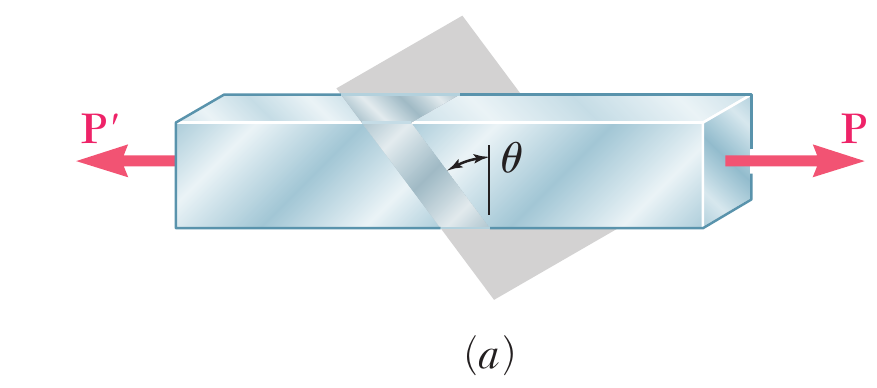
\includegraphics[width=\linewidth,height=1.5cm,keepaspectratio]{Chap_1/fig_1_28a.png}\\[2pt]
      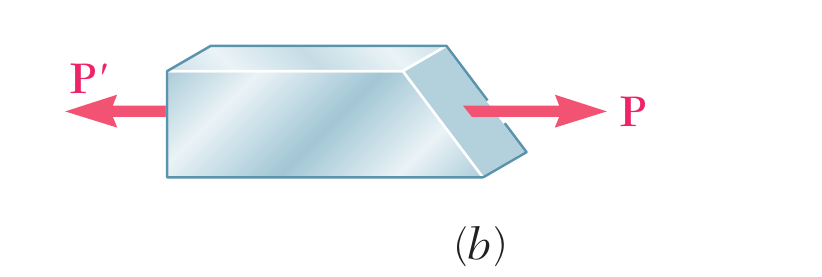
\includegraphics[width=\linewidth,height=1.5cm,keepaspectratio]{Chap_1/fig_1_28b.png}\\[2pt]
      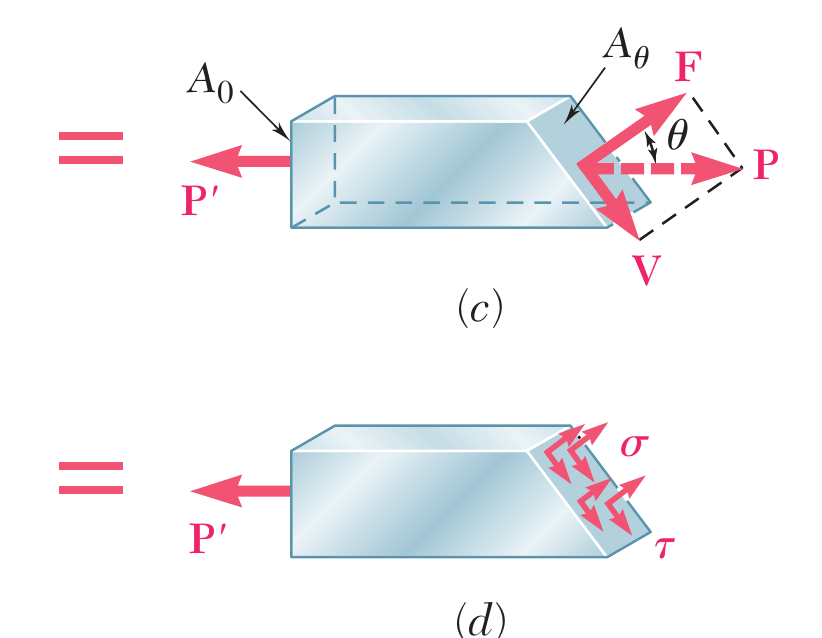
\includegraphics[width=\linewidth,height=3cm,keepaspectratio]{Chap_1/fig_1_28cd.png}
    \column{0.62\textwidth}
      \footnotesize
      \begin{itemize}
        \setlength{\itemsep}{0.4em}
        \item Cắt cấu kiện bằng một mặt cắt hợp với mặt cắt ngang (vuông
              góc với trục) một góc $\theta$.
        \item Từ điều kiện cân bằng, các lực phân bố (ứng suất) trên mặt
              cắt phải tương đương với lực $P$.
        \item Phân tích $P$ thành các thành phần pháp tuyến và tiếp tuyến
              với mặt cắt nghiêng:
        \[
          F = P\cos\theta, \qquad V = P\sin\theta
        \]
        \item Ứng suất pháp và ứng suất tiếp trung bình trên mặt cắt
              nghiêng:
        \[
          \sigma = \frac{F}{A_\theta}
                 = \frac{P\cos\theta}{A_0/\cos\theta}
                 = \frac{P}{A_0}\cos^2\theta
        \]
        \[
          \tau = \frac{V}{A_\theta}
               = \frac{P\sin\theta}{A_0/\cos\theta}
               = \frac{P}{A_0}\sin\theta\cos\theta
        \]
      \end{itemize}
  \end{columns}
\end{frame}
% ===========
\section{Ứng suất lớn nhất}
\begin{frame}[t]{Ứng suất lớn nhất}
  \begin{columns}[T]
    \column{0.36\textwidth}
      \centering
      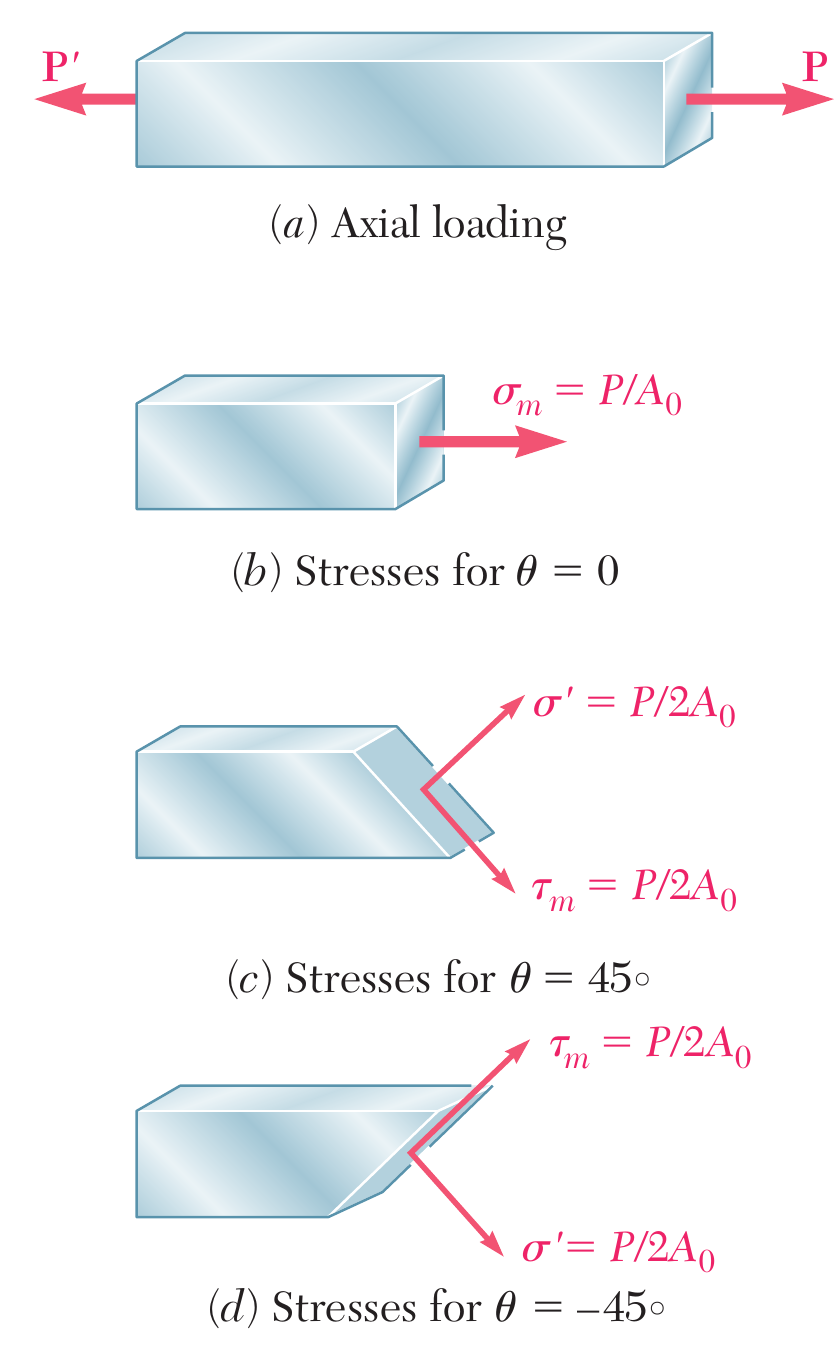
\includegraphics[width=\linewidth,height=6.5cm,keepaspectratio]{Chap_1/fig_1_29.png}
    \column{0.62\textwidth}
      \small
      \begin{itemize}
        \setlength{\itemsep}{0.6em}
        \item Ứng suất pháp và ứng suất tiếp trên mặt cắt nghiêng:
        \[
          \sigma = \frac{P}{A_0}\cos^2\theta \qquad
          \tau = \frac{P}{A_0}\sin\theta\cos\theta
        \]
        \item Ứng suất pháp lớn nhất xuất hiện khi mặt cắt vuông góc với
              trục cấu kiện ($\theta = 0$):
        \[
          \sigma_m = \frac{P}{A_0}, \qquad \tau' = 0
        \]
        \item Ứng suất tiếp lớn nhất xuất hiện trên mặt cắt nghiêng
              $\pm 45^\circ$ so với trục:
        \[
          \tau_m = \frac{P}{A_0}\sin 45^\circ\cos 45^\circ
                 = \frac{P}{2A_0} = \sigma'
        \]
      \end{itemize}
  \end{columns}
\end{frame}
% ===========
\section{Ứng suất dưới tác dụng của tải trọng tổng quát}
\begin{frame}[t]{Ứng suất dưới tác dụng của tải trọng tổng quát}
  \begin{columns}[T]
    \column{0.40\textwidth}
      \centering
      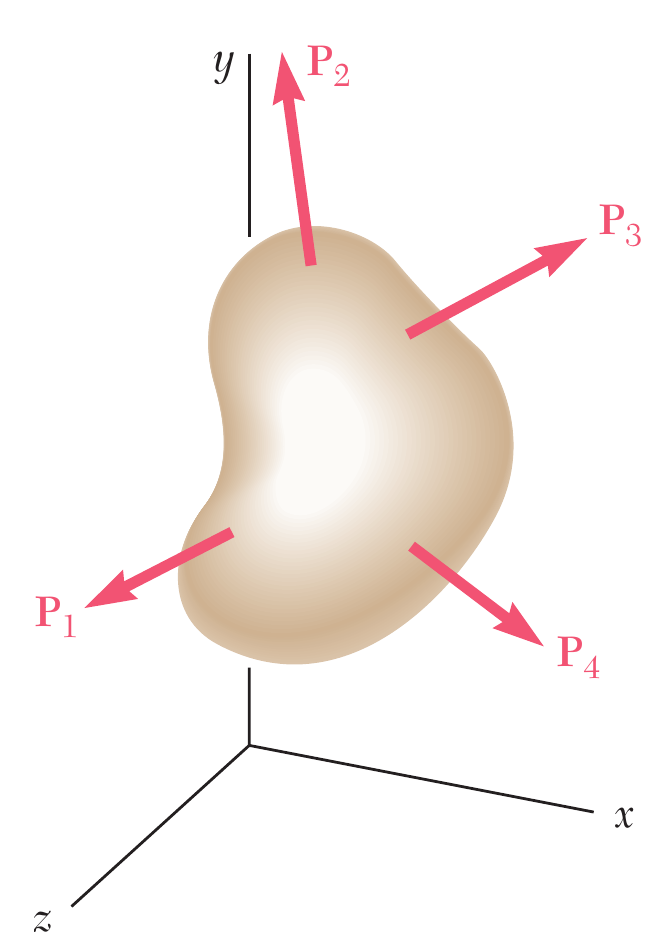
\includegraphics[width=\linewidth,height=3.5cm,keepaspectratio]{Chap_1/fig_1_30.png}\\[2pt]
      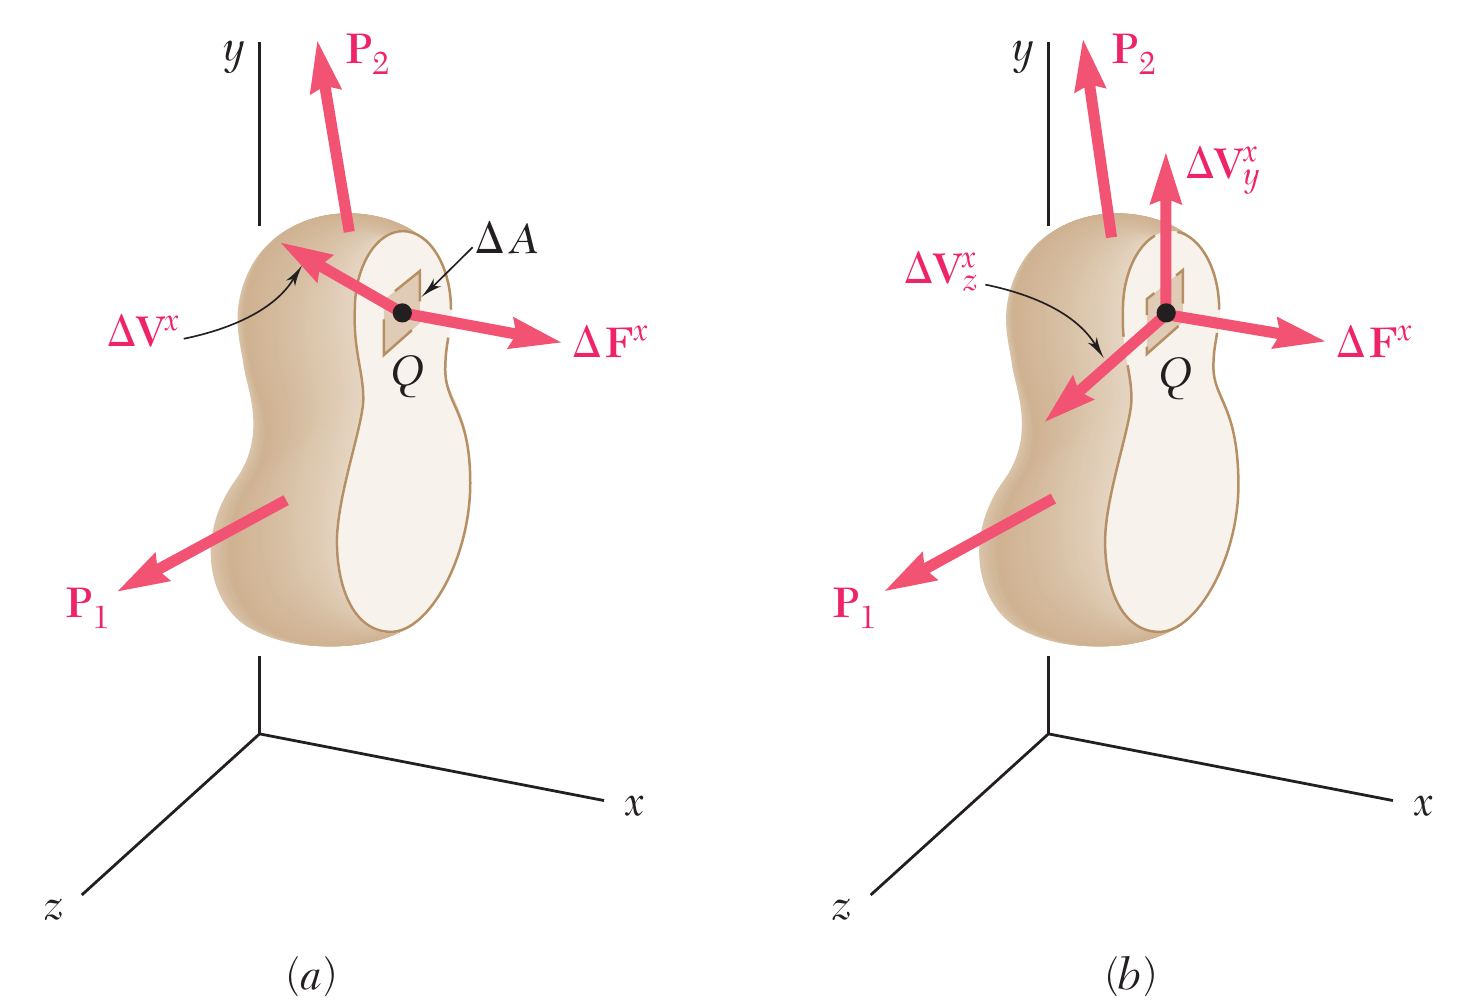
\includegraphics[width=\linewidth,height=3.2cm,keepaspectratio]{Chap_1/fig_1_31.png}
    \column{0.58\textwidth}
      \small
      \begin{itemize}
        \setlength{\itemsep}{0.6em}
        \item Cấu kiện chịu tổ hợp tải trọng tổng quát được cắt thành
              hai phần bởi một mặt phẳng đi qua điểm $Q$.
        \item Phân bố các thành phần ứng suất bên trong có thể được định
              nghĩa như sau:
        \[
          \sigma_x = \lim_{\Delta A\to 0}\frac{\Delta F^x}{\Delta A}
        \]
        \[
          \tau_{xy} = \lim_{\Delta A\to 0}\frac{\Delta V_y^x}{\Delta A}
          \qquad
          \tau_{xz} = \lim_{\Delta A\to 0}\frac{\Delta V_z^x}{\Delta A}
        \]
        \item Để cân bằng, phần còn lại của cấu kiện phải chịu một phân
              bố nội lực và ứng suất bằng và ngược chiều.
      \end{itemize}
  \end{columns}
\end{frame}
% ===========
\section{Trạng thái ứng suất}
\begin{frame}[t]{Trạng thái ứng suất}
  \begin{columns}[T]
    \column{0.36\textwidth}
      \centering
      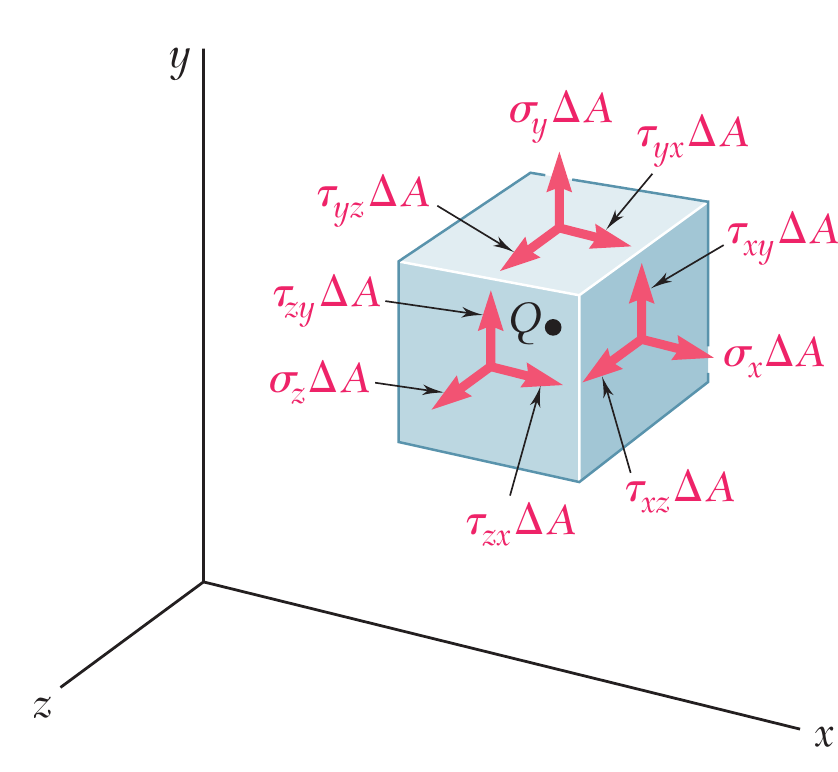
\includegraphics[width=\linewidth,height=2.9cm,keepaspectratio]{Chap_1/fig_1_35.png}\\[2pt]
      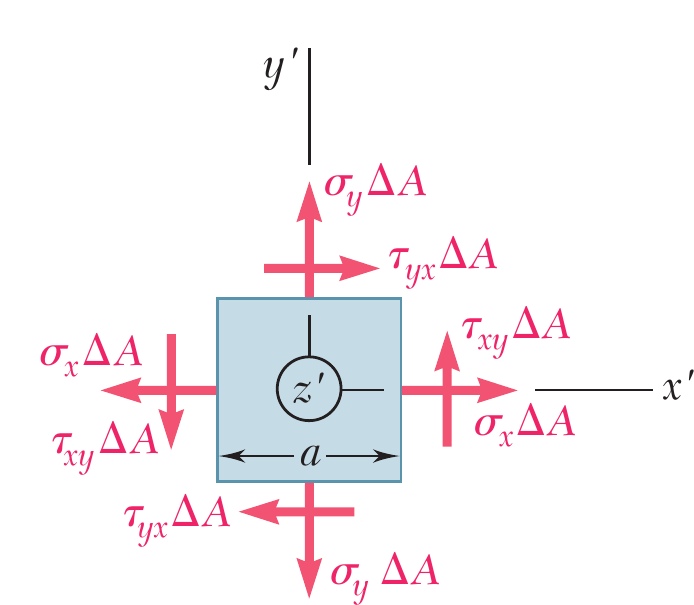
\includegraphics[width=\linewidth,height=3.5cm,keepaspectratio]{Chap_1/fig_1_36.png}
    \column{0.62\textwidth}
      \footnotesize
      \begin{itemize}
        \setlength{\itemsep}{0.4em}
        \item Các thành phần ứng suất được định nghĩa trên các mặt cắt
              song song với các trục $x$, $y$, $z$. Các ứng suất bằng và
              ngược chiều tác dụng trên các mặt khuất.
        \item Tổ hợp các lực sinh ra bởi các ứng suất phải thỏa mãn điều
              kiện cân bằng:
        \[
          \textstyle\sum F_x = \sum F_y = \sum F_z = 0, \qquad
          \sum M_x = \sum M_y = \sum M_z = 0
        \]
        \item Xét mô men đối với trục $z$:
        \[
          \textstyle\sum M_z = 0 = (\tau_{xy}\Delta A)a - (\tau_{yx}\Delta A)a
          \quad\Rightarrow\quad \tau_{xy} = \tau_{yx}
        \]
        tương tự: $\tau_{yz} = \tau_{zy}$ và $\tau_{zx} = \tau_{xz}$.
        \item Suy ra chỉ cần 6 thành phần ứng suất để xác định hoàn toàn
              trạng thái ứng suất tại một điểm.
      \end{itemize}
  \end{columns}
\end{frame}
% ===========
\section{Hệ số an toàn}
\begin{frame}[t]{Hệ số an toàn}
  \begin{columns}[T]
    \column{0.44\textwidth}
      \small
      \begin{itemize}
        \setlength{\itemsep}{0.6em}
        \item Cấu kiện kết cấu hoặc máy phải được thiết kế sao cho ứng
              suất làm việc nhỏ hơn giới hạn bền của vật liệu.
        \item Hệ số an toàn:
        \[
          FS = \frac{\sigma_u}{\sigma_{\mathrm{all}}}
             = \frac{\text{giới hạn bền}}{\text{ứng suất cho phép}}
        \]
      \end{itemize}
    \column{0.54\textwidth}
      \small
      Các yếu tố cần xem xét khi chọn hệ số an toàn:
      \begin{itemize}
        \setlength{\itemsep}{0.2em}
        \item độ không chắc chắn về đặc tính vật liệu
        \item độ không chắc chắn về tải trọng
        \item độ không chắc chắn của phép phân tích
        \item số chu kỳ chịu tải
        \item các dạng phá hủy
        \item yêu cầu bảo dưỡng và ảnh hưởng của sự xuống cấp
        \item tầm quan trọng của cấu kiện đối với sự toàn vẹn của kết cấu
        \item rủi ro đối với con người và tài sản
        \item ảnh hưởng đến chức năng của máy
      \end{itemize}
  \end{columns}
\end{frame}

\end{document}
